\documentclass[conference]{IEEEtran}
\IEEEoverridecommandlockouts
% The preceding line is only needed to identify funding in the first footnote. If that is unneeded, please comment it out.
\usepackage{cite}
\usepackage{amsmath,amssymb,amsfonts}
\usepackage{algorithmic}
\usepackage{graphicx}
\usepackage{textcomp}
\PassOptionsToPackage{hyphens}{url}\usepackage{hyperref}
\usepackage{xcolor,colortbl}
\usepackage{dblfloatfix}
\newcommand{\cbox}[1]{\raisebox{\depth}{\fcolorbox{black}{#1}{\null}}}
\newcommand{\n}{\hfill\break}
\usepackage{svg}


\hypersetup{
	colorlinks,
	linkcolor={red!50!black},
	citecolor={green!75!black},
	urlcolor={blue!80!black}
}
\def\BibTeX{{\rm B\kern-.05em{\sc i\kern-.025em b}\kern-.08em
    T\kern-.1667em\lower.7ex\hbox{E}\kern-.125emX}}
\begin{document}

\title{A Primer on the Metallic Arts}

\author{\IEEEauthorblockN{McDonald, J}
\IEEEauthorblockA{
Honolulu, HI \\
@jamcdonald120}
}

\maketitle

\begin{abstract}
In the Cosmere there are 3 interlocked investiture Hemalurgy, Feruchemy, and Allomancy.  These systems have such a large influence on the Cosmere as a whole that they can not go ignored despite being mostly confined to Scadrial.  Additionally Rosharan fabrial technology appears to use the same metals, further increasing influence.
\end{abstract}

\begin{IEEEkeywords}
meta, Brandon Sanderson, Mistborn: The Final Empire, Mistborn: Well of Ascension, Mistborn: Hero of Ages, Mistborn: Bands of Mourning, Mistborn: The 11th metal, Mistborn: The Secret History, Mistborn: The Alloy of Law, Mistborn: Shadows of Self, Mistborn, Fabrial Tech
\end{IEEEkeywords}

\section*{Introduction}
Allomancy, Feruchemy, and Hemalurgy all use the same 16 base metals and some ``God metals" created by shards.\cite{ARS} Due to the nature of the systems they are interlocked not only with each other, but with all other investiture systems in the entire Cosmere.  As an example of their combined power, a Scadrian (the Lord Ruler) with access to all 3 became a functionally immortal demigod king with a 1000 year reign.\cite{TFE}  The only non vessel, non splinter, humanoids who have achieved this level of power are Hoid, and possibly Vasher.  As such, the basics of these 3 systems are critical to understanding the Cosmere as a whole.  Additionally Rosharan fabrial tech appears to use the same metals,\cite{RoW-E7} however not all base metals have a known use in fabrial tech yet, and may be currently undiscovered on Roshar. 

The purpose of this paper is mostly to consolidate existing knowledge and to act as a single point of reference for future papers working with the metallic arts.  There is some Limited speculation as well.
\section*{The very basics}
\subsection*{Allomancy}
All Allomancers draw power through various metals through a process called ``burning".\cite{TFE-CH7}  The Allomancer ingests a quantity of a specific metal and then can ``burn" the metal to channel power from the shard Preservation\cite{allo-source}.  The metal is destroyed in the process and vast amounts of investiture are released.  The exact nature of this investiture depends on the metal its self\cite{TFE-CH7} as will be explored in more detail in a later section.  A metal can be ``flared" or burned faster to produce a limited boost in power, but there is an upper limit to how fast an individual can burn a metal.  Each metal and its alloy are ``paired" and have related effects, one being classified as pushing, and the other as pulling.\cite{TFE-CH7}
\subsection*{Feruchemy}
A Feruchemist can store various attributes in various metals, temporarily loosing part of that attribute in themselves.\cite{TFE-CH22}   This creates a ``metalmind".  Later the Feruchemist can withdraw any attributes they have stored within a metalmind to gain a boost to that attribute.  Feruchemy is mostly net neutral.  The amount of attribute stored is effectively the amount that can be withdrawn, minus a slight degradation from inefficiencies.  The attribute that can be stored depends on which metal the metalmind is composed of.\cite{TFE-CH22}  The Feruchemist can withdraw any amount of stored investiture at any rate.  This means given enough time, a Feruchemist can have access to far more investiture at once than an Allomancer can.\cite{TFE-CH27}
While a Feruchemist can store and withdraw any amount of invested attribute at any given time (so long as the reserve is there), there is an optimal rate for both, storing or withdrawing faster than this rate results in compounding levels of inefficiencies.  So while a Feruchemist may be able to store 50\% of an attribute to access 150\% for a similar time, the time the Feruchemist could access the reserve at 200\% would be less than half as long, despite the Feruchemist drawing exactly twice as much of the attribute.\cite{fe-decay}

In most cases, a metalmind is identity locked to its creator and can not be used by another person, however there are 2 special types of metalminds unsealed, and unkeyed which will be addressed later.\cite{BoM-CH3} 
\subsection*{Hemalurgy}
Hemalurgy is a unique and complicated system and can only be fully utilized by someone with a mind as vast as a shard.\cite{WoF}  Hemalurgy has 3 modes of operation, the first mode is theft.  For theft, a metal spike is driven into the body of a victim at specific bind point with intent will steal an ability.\cite{WoF}  The attribute stolen depends on the metal\cite{WoF}, bind point\cite{WoB-holiday}, and intent\cite{HE-intent} that used.  The resulting attribute permanently binds it to the spike creating a Hemalurgic spike.\cite{ARS}  This process usually kills the ``donor" but does not require death to function,\cite{noDeath} only that the spike touches blood in a bind point.  The spike will lose investiture any time it is outside of a body, although it will never completely discharge.\cite{HoA-CH34}\cite{WoF}  This can be mitigated somewhat by storing the spike in Aluminum\cite{anti-decay-aluminum} or blood,\cite{anti-decay-blood} but loss of investiture is an innate part of Hemalurgy.\cite{WoF}  Only 1 attribute can be stolen from a person,\cite{HE-only1} and the stolen attribute will always be weaker than it was in the person.\cite{HoA-CH34}  Some metals can various attributes, the exact attribute stolen is dependent on the bind point\cite{WoB-holiday} and intent\cite{HE-intent} used, however no specific bind point effect is known.
Each metal and bind point has a different effect.  The attribute stolen depends on both the metal and bind point used\cite{WoF}.  It is possible for any investiture system tied to a persons spirit web to be stolen by Hemalurgy, but the exact metals and bind points are only known for Feruchemy and Allomancy.\cite{HE-universal}  Very little is known about the bind points and their significance.

Once a Hemalurgic spike has been created, the 2nd and 3rd mode of operation are possible.  If a Hemalurgic spike is then driven into another person, that person gains access to the ability stored within the spike.\cite{ARS}  Driving this spike correctly will not kill the person even if the spike is placed in a normally fatal manner, such as through the heart or brain.\cite{TFE-CH2}  However, an improperly prepared Spike or an insertion at an incorrect bind point CAN kill.  Vital organs will rearrange to accommodate the spike,\cite{WoF} and the spike insertion point can not become infected.\cite{noInfect}  Removal of a spike placed in such a way can kill its bearer.\cite{HoA-CH42}  

The 3rd mode of operation is some what more complex.  It is possible to create unique entities with Hemalurgic spikes.\cite{WoF}  Only 4 such entity templates are known to exist, 3 where created by Rashek while holding the power of preservation,\cite{WoF} and the 4th by an unknown shard working through a Kandra.\cite{SoS-CH21} 

Hemalurgy caries inherent risk, each spike placed in an entity increases its vulnerability to shards and other mental influences.\cite{HE-Shard}\cite{HoA-CH58}\cite{HoA-CH13}\cite{HoA-CH77}  For example, even with a single spike, Preservation can hear your thoughts,\cite{SoS-CH7} and Ruin can speak in your mind.\cite{HoA-CH65}  As few as 2 spikes have been shown to allow a shard to take complete control of an individual,\cite{SoS-CH7} although the lower limit for a shard controlling a non-construct is 4.\cite{BoM-CH27}  It is suggested there is a way to benefit from Hemalurgy, but transfer these vulnerabilities to another.\cite{BoM-CH27}  The exact method of doing so is unknown, most likely it involves manipulating identity or connection in some way.
\subsection*{Fabrial Tech}
Fabrial tech also has a substantial overlap in the metals it uses.\cite{RoW-E7}  This paper will touch on the effects of specific metals within Fabrial tech, but is not a comprehensive guide to Fabrials and will not address anything else about their construction.
%I hate latex, this table has to go here to appear where I actually want it%
\begin{table*}[!hb]
	
	\caption{Table of Metals}
	\centering
	\begin{tabular}{ |l |ccc c ccc | ccc c ccc | r| }
		\hline
		Physical&&Push&&&&Pull&&&Pull&&&&Push&&Mental/Cognitive\\\hline
		External&
\includegraphics[height=1em]{images/Steel.png}& Steel & 
\includegraphics[height=1em]{images/Steel_(Feruchemy).png}&&
\includegraphics[height=1em]{images/Iron.png}& Iron& 
\includegraphics[height=1em]{images/Iron_(Feruchemy).png}&
\includegraphics[height=1em]{images/Zinc.png} &Zinc& 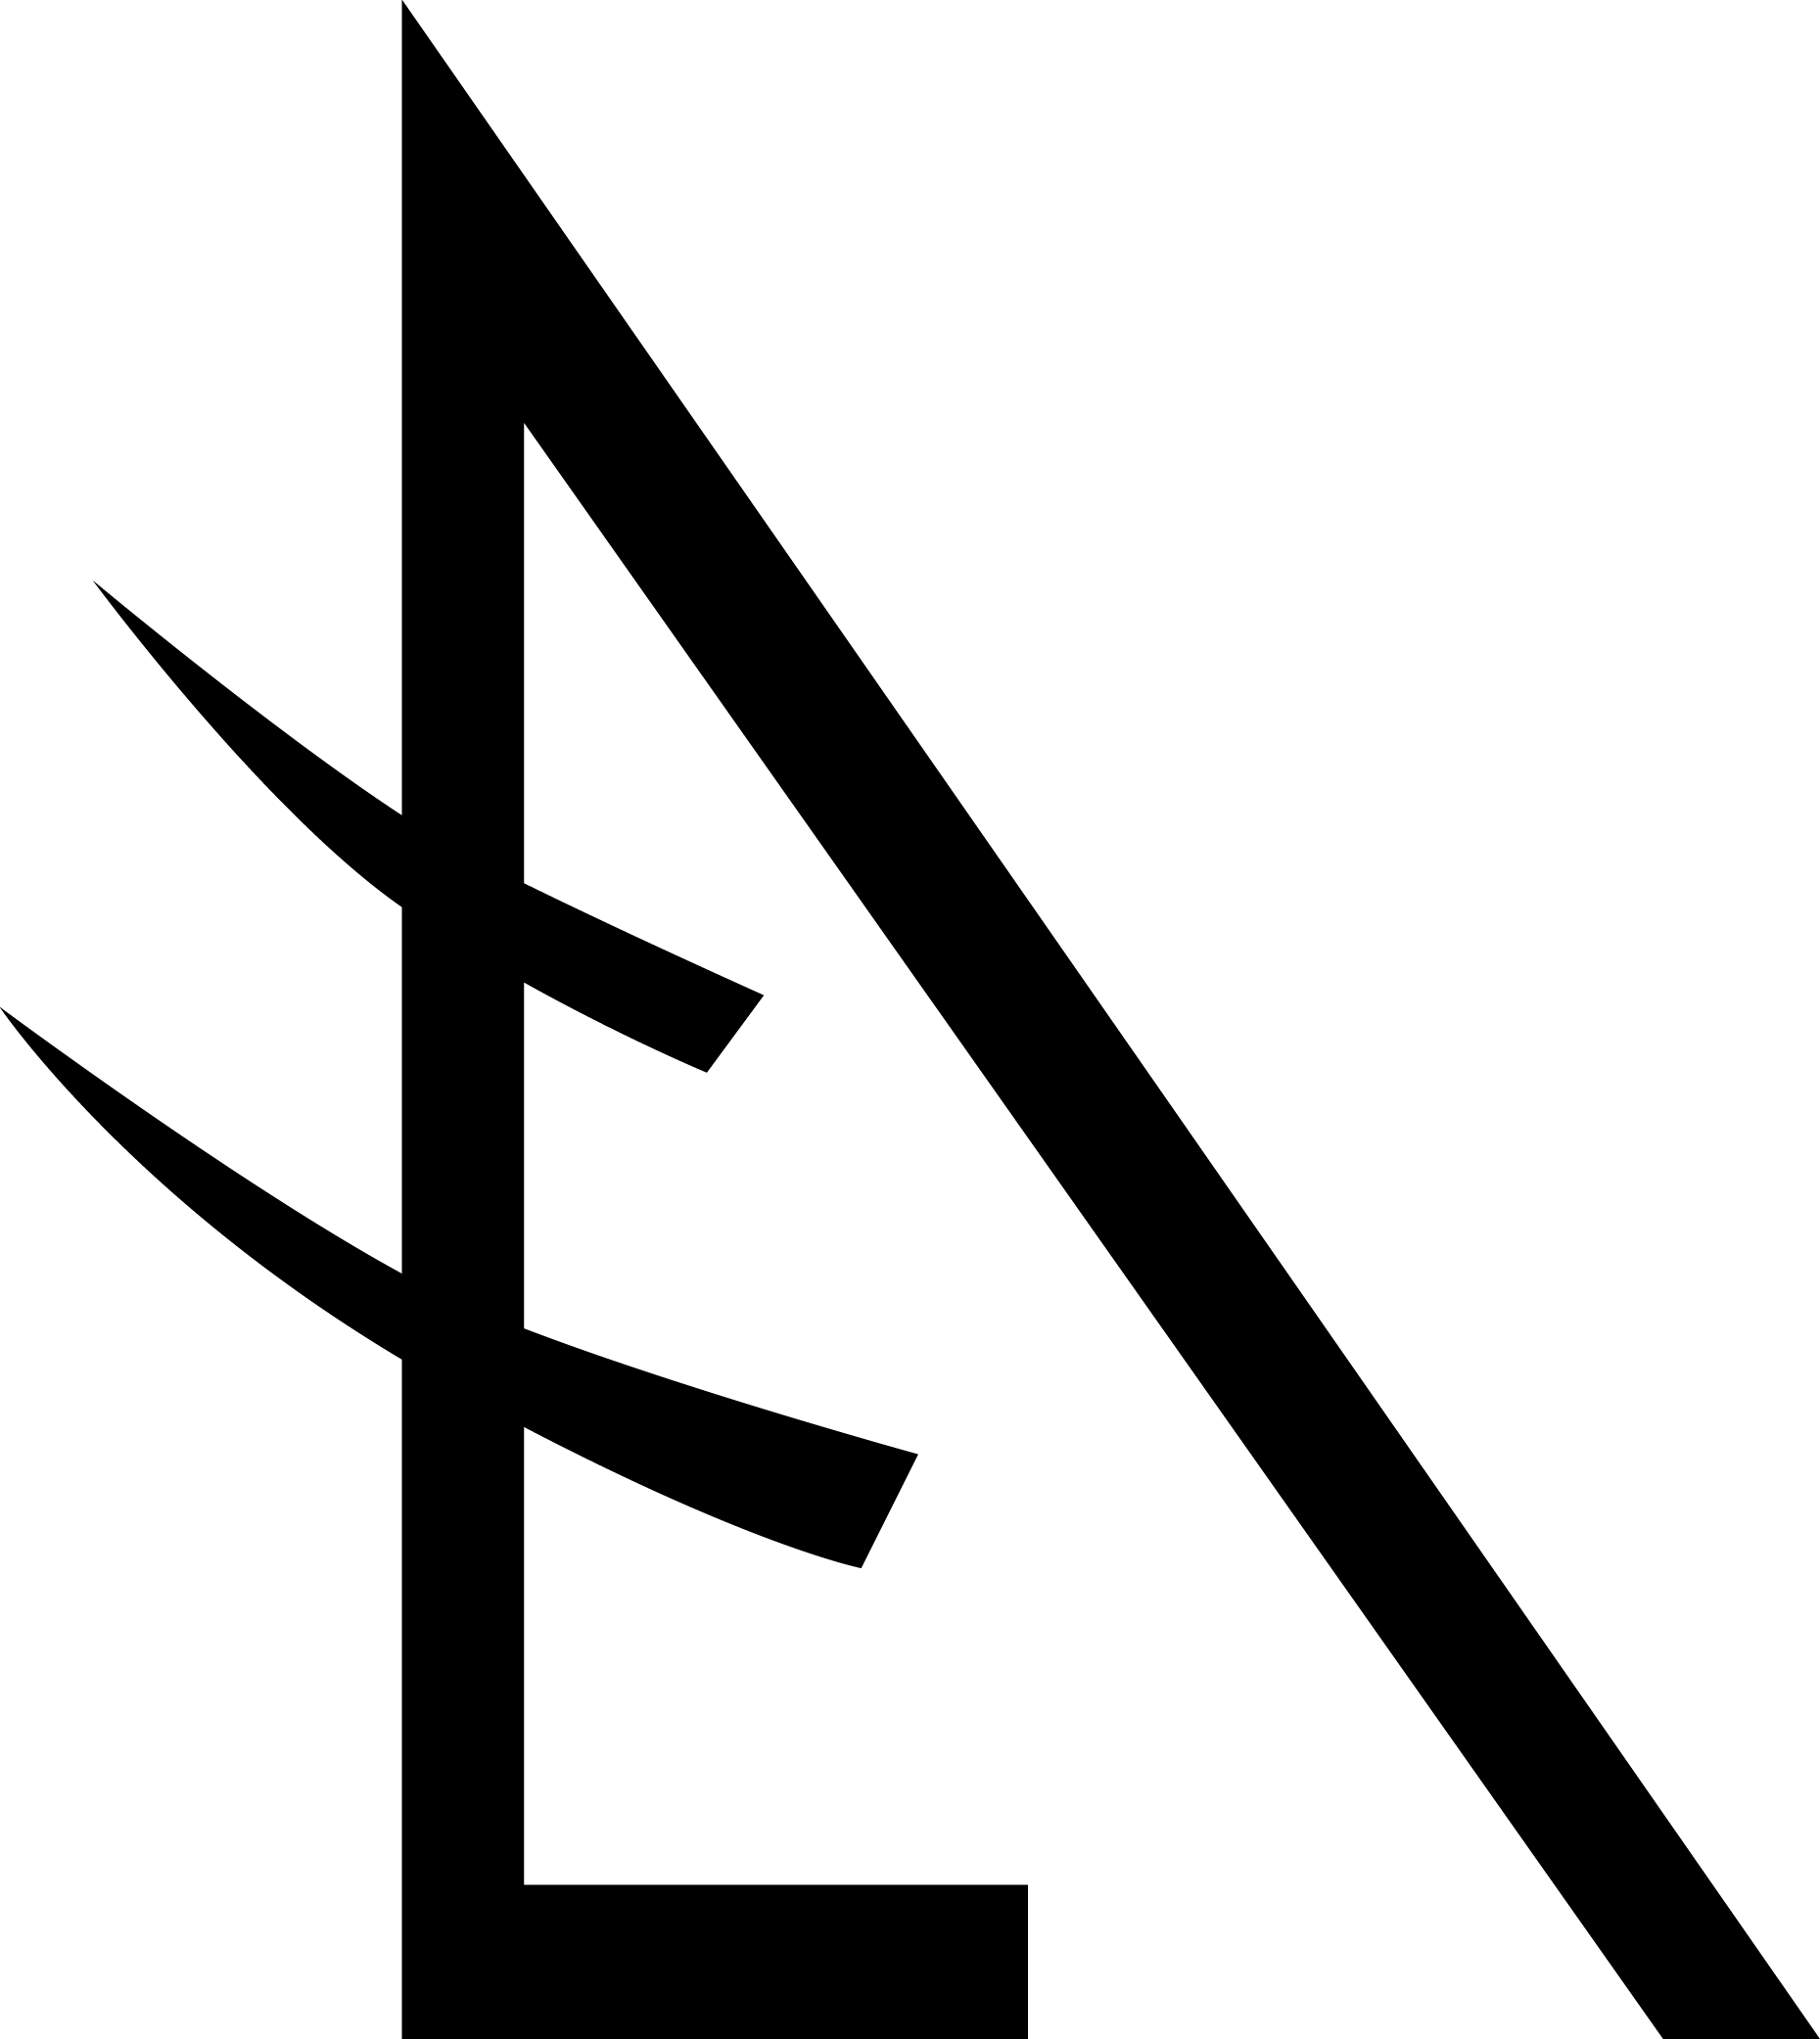
\includegraphics[height=1em]{images/Zinc_(Feruchemy).png}&&
\includegraphics[height=1em]{images/Brass.png}& Brass& 
\includegraphics[height=1em]{images/Brass_(Feruchemy).png}&External\\
		Internal&
\includegraphics[height=1em]{images/Pewter.png} &Pewter& 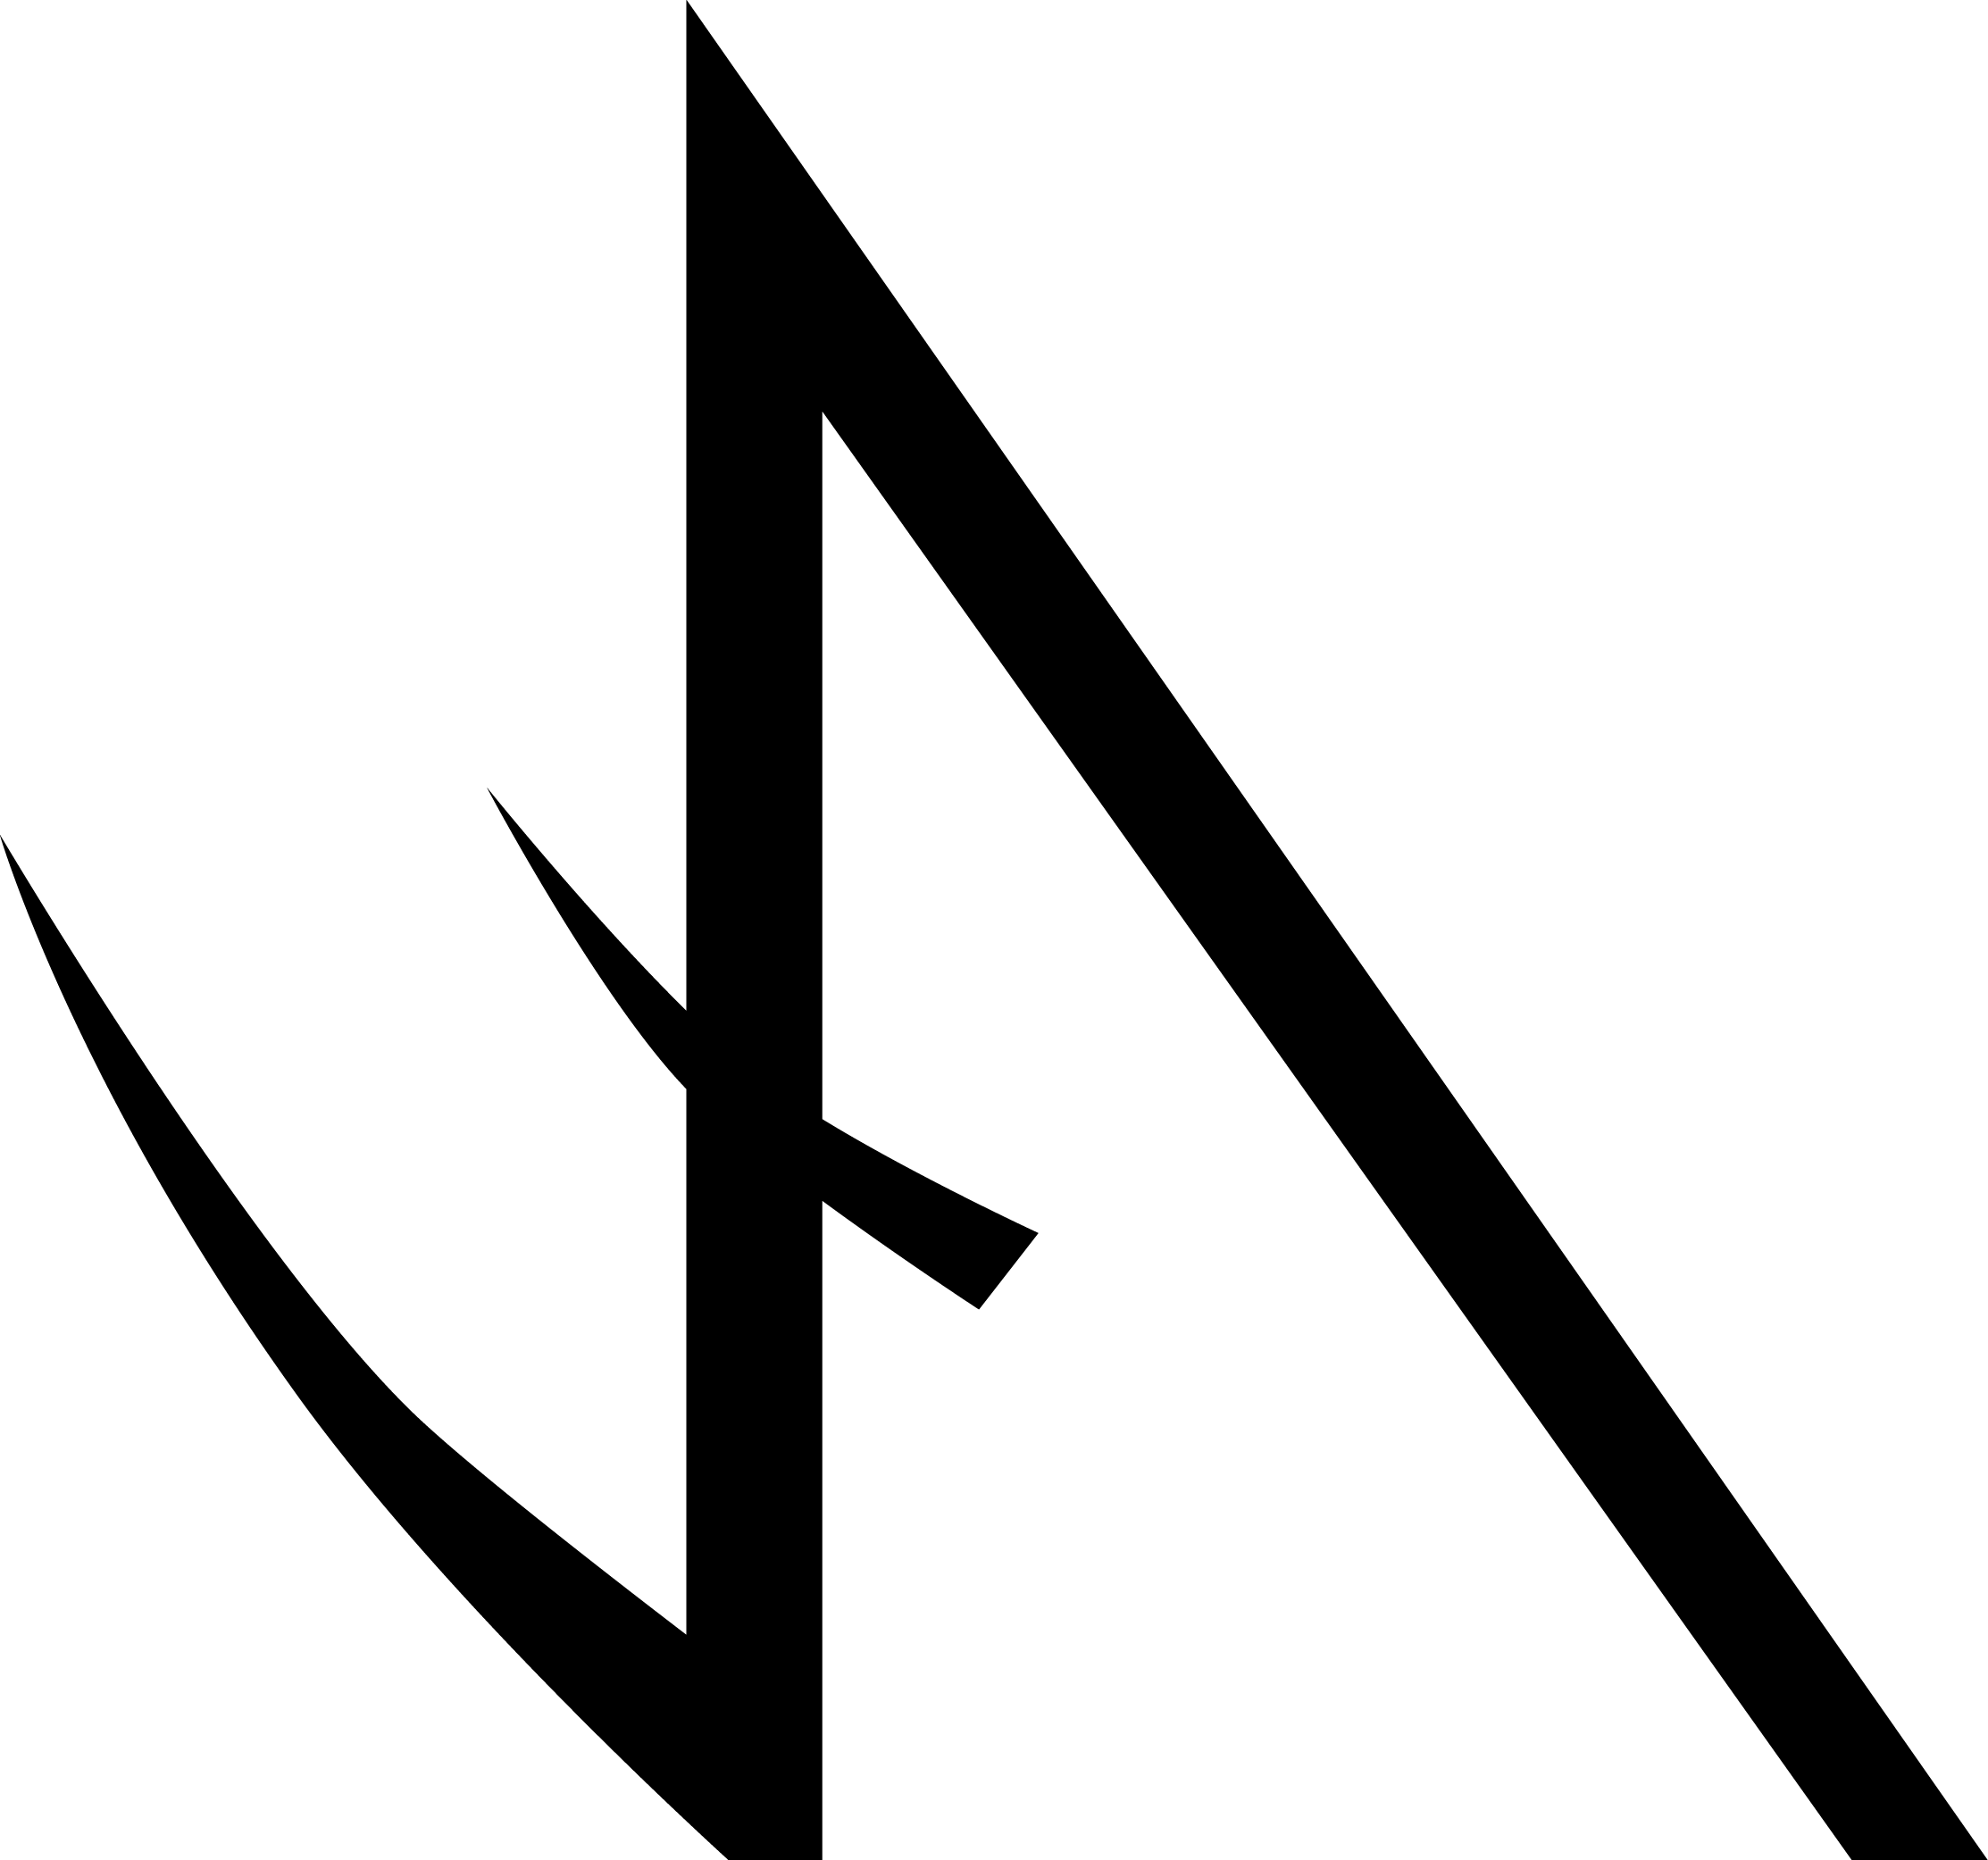
\includegraphics[height=1em]{images/Pewter_(Feruchemy).png}&&
\includegraphics[height=1em]{images/Tin.png} &Tin& 
\includegraphics[height=1em]{images/Tin_(Feruchemy).png}&
\includegraphics[height=1em]{images/Copper.png} &Copper& 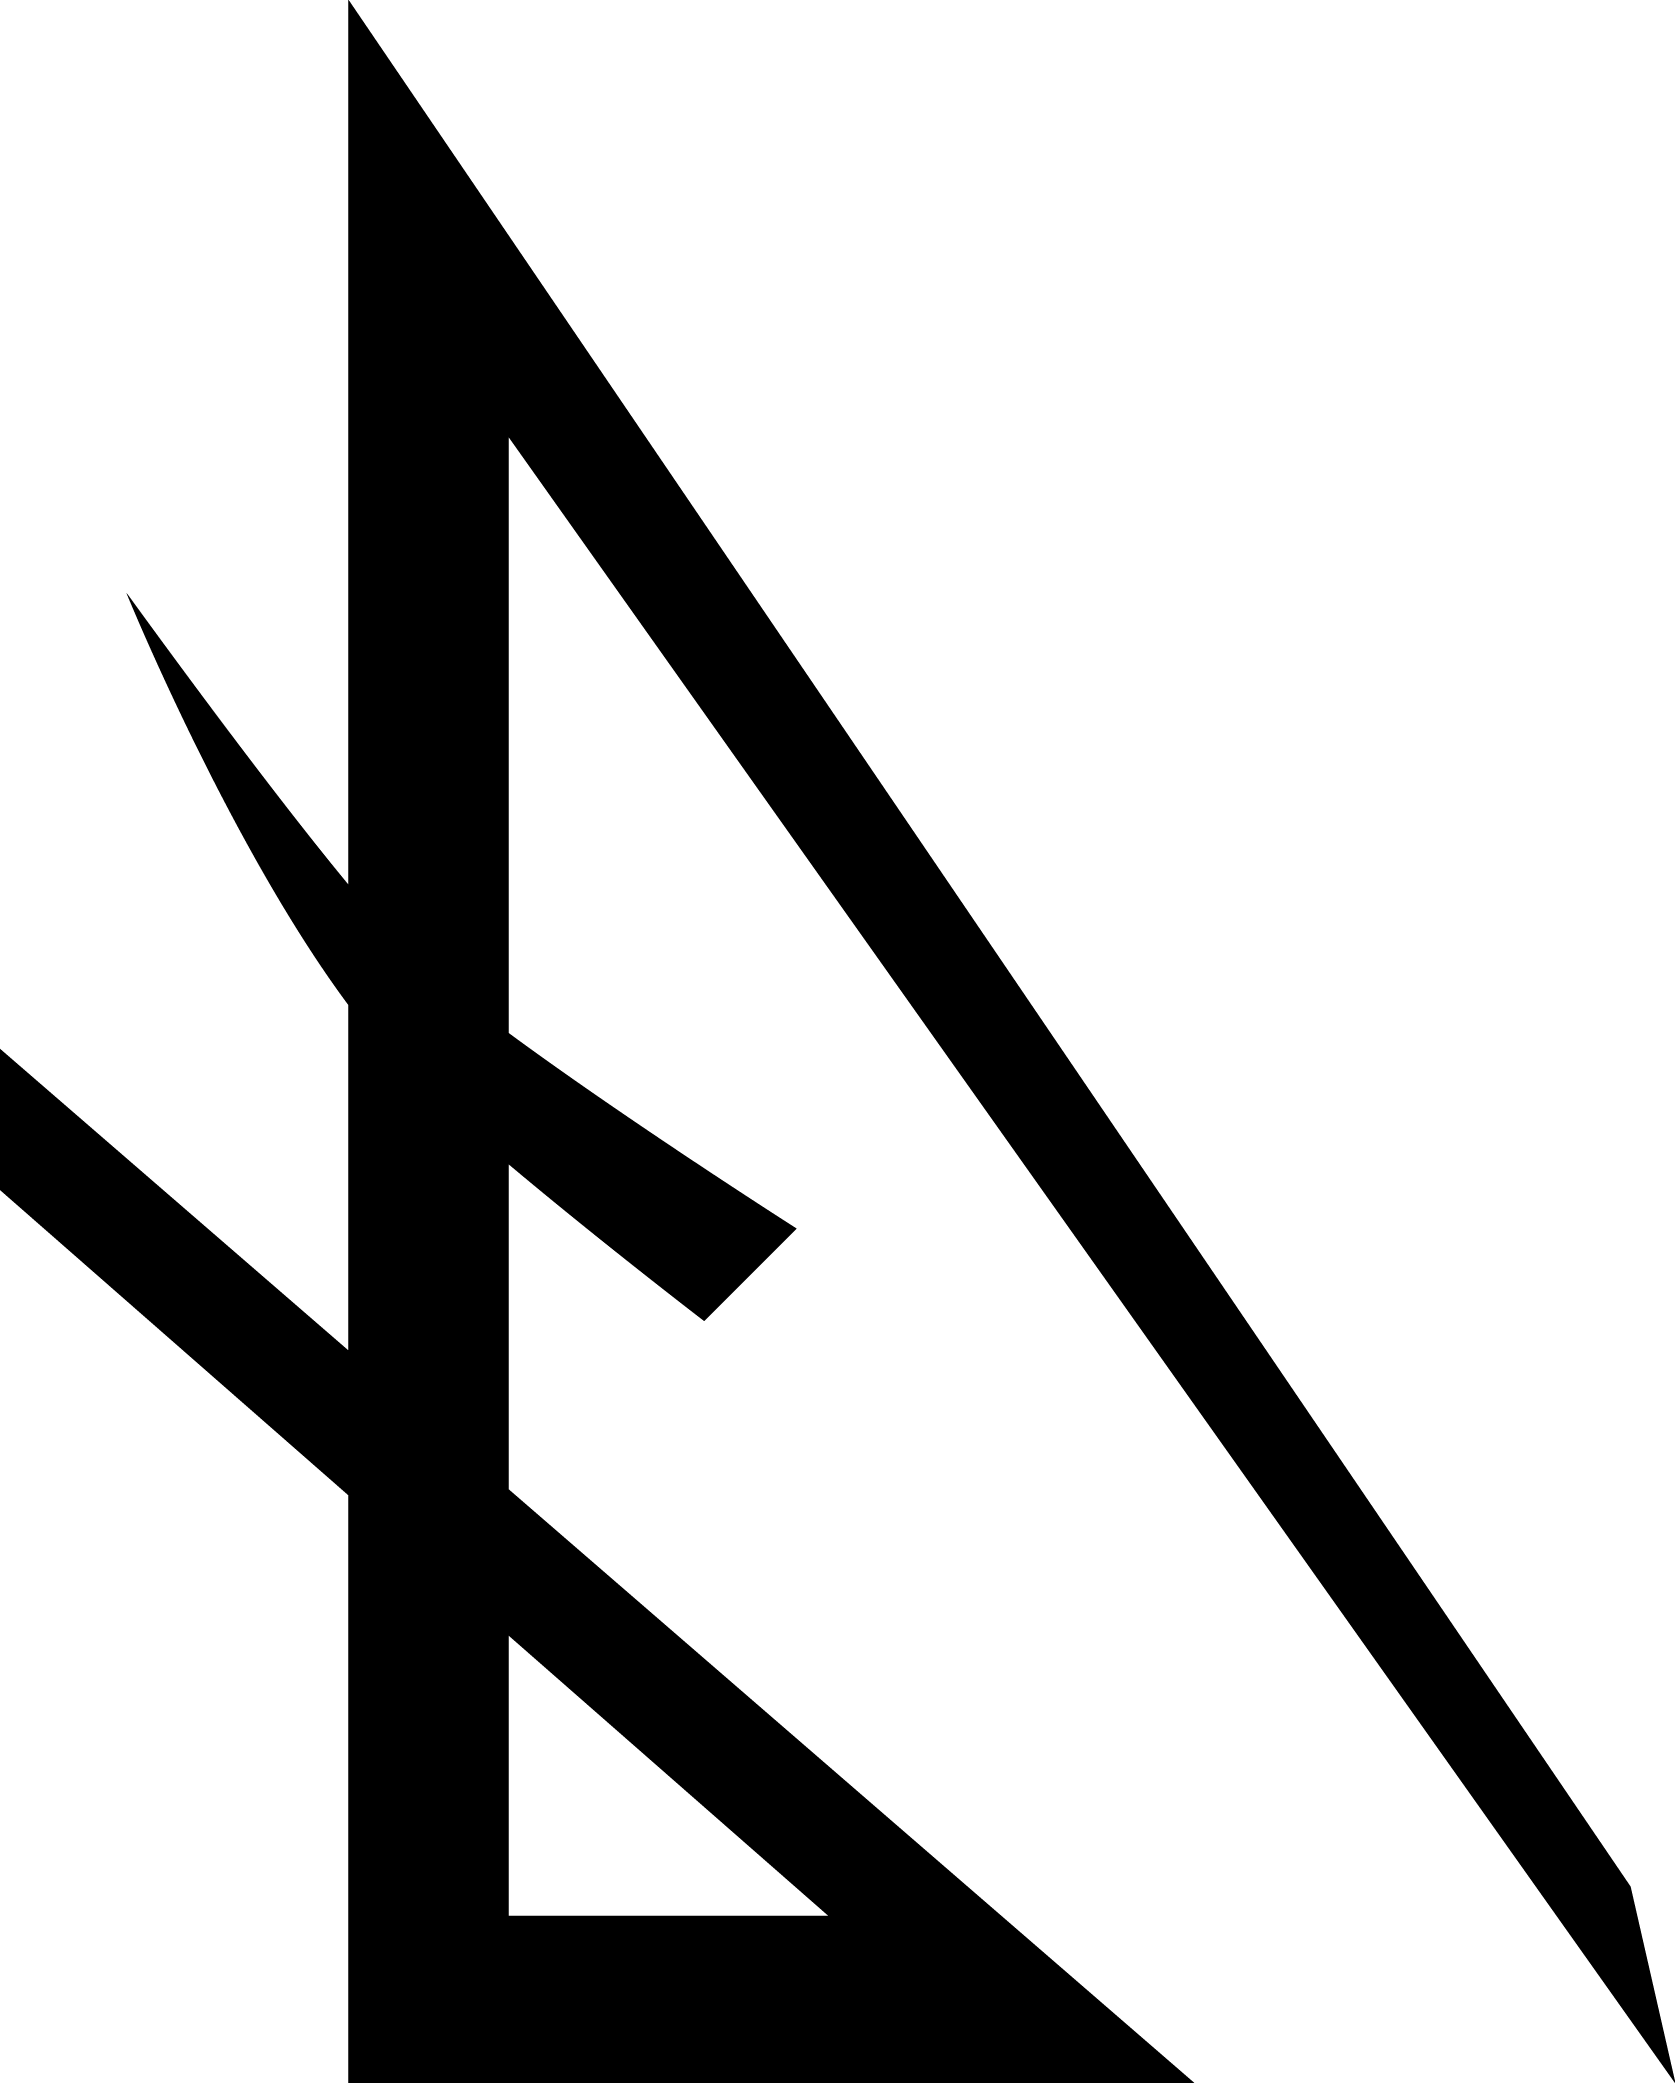
\includegraphics[height=1em]{images/Copper_(Feruchemy).png}&&
\includegraphics[height=1em]{images/Bronze.png}& Bronze& 
\includegraphics[height=1em]{images/Bronze_(Feruchemy).png}&Internal\\
		\hline
		Internal&
\includegraphics[height=1em]{images/Duralumin.png} &Duralumin& 
\includegraphics[height=1em]{images/Duralumin_(Feruchemy).png}&&
\includegraphics[height=1em]{images/Aluminum.png}& Aluminum& 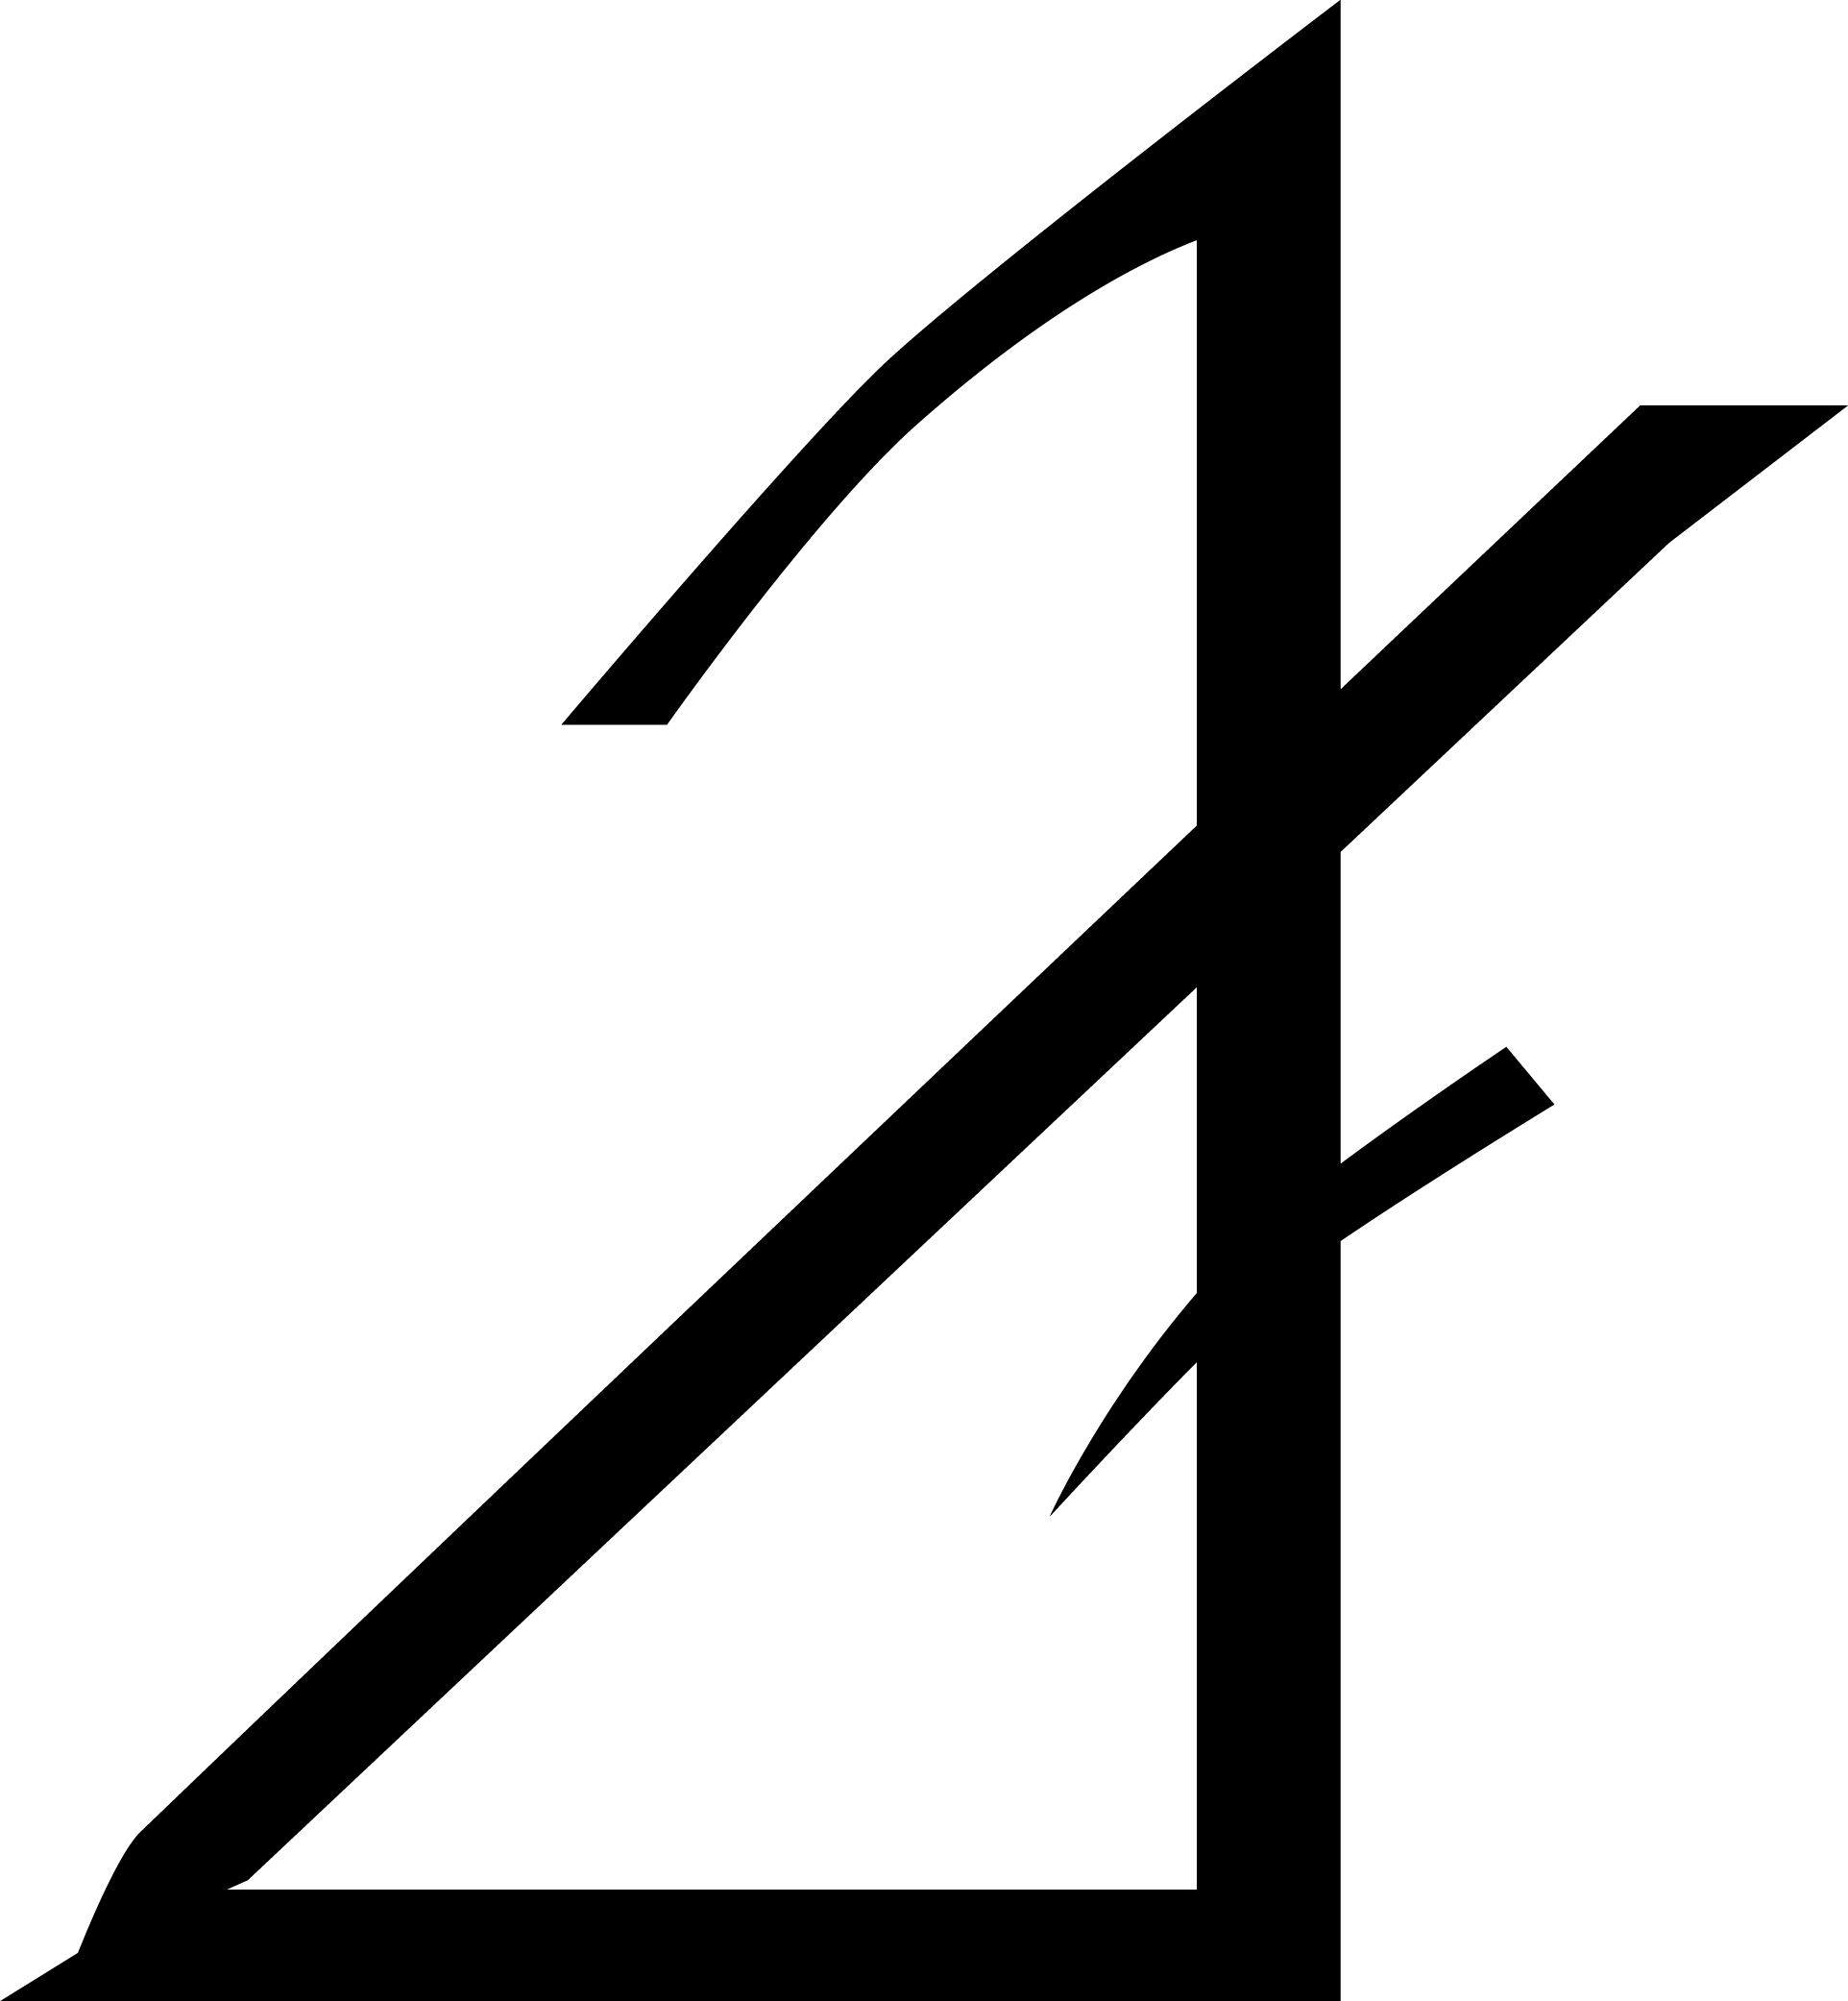
\includegraphics[height=1em]{images/Aluminum_(Feruchemy).png}&
\includegraphics[height=1em]{images/Gold.png}& Gold& 
\includegraphics[height=1em]{images/Gold_(Feruchemy).png}&&
\includegraphics[height=1em]{images/Electrum.png} &Electrum&
\includegraphics[height=1em]{images/Electrum_(Feruchemy).png}&Internal\\
		External&
\includegraphics[height=1em]{images/Nicrosil.png} &Nicrosil& 
\includegraphics[height=1em]{images/Nicrosil_(Feruchemy).png}&&
\includegraphics[height=1em]{images/Chromium.png}& Chromium& 
\includegraphics[height=1em]{images/Chromium_(Feruchemy).png}&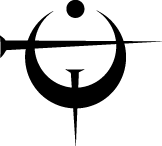
\includegraphics[height=1em]{images/Cadmium.png} &Cadmium& 
\includegraphics[height=1em]{images/Cadmium_(Feruchemy).png}&&
\includegraphics[height=1em]{images/Bendalloy.png}& Bendalloy& 
\includegraphics[height=1em]{images/Bendalloy_(Feruchemy).png}&External\\\hline
		Enhancement/Spiritual&&Push&&&&Pull&&&Pull&&&&Push&&Temporal/Hybrid\\\hline
	\end{tabular}
\vspace{0.5em}\break
Each metal has an associated Allomantic\cite{AL-TB} (left) and Feruchemical\cite{FE-TB} (right) symbol
	\label{metals}
\end{table*}
\hfill
\section*{Classifications of Users}

\subsection*{Allomancy}
A person who can use only 1 base metal is called a Misting.\cite{TFE-CH3}  Anyone who can use 2 base metals on their own can use ALL metals and is called a Mistborn.  It is possible to become Allomancers either by being born one,\cite{TFE-CH3} or by ingesting a bead of Lerasium.\cite{WoA-CH59}  Before a genetic Allomancer can know they have any ability, they must suffer a near death experience known as snapping.\cite{TFE-CH17}  This can be a brutal beating, a bad illness, or similar.  Someone holding preservation power can also make someone an Allomancer,\cite{HoA-EP} it is unknown if other shards can do this as well.  There are different skill and power levels among Allomancers,\cite{WoA-CH54}\cite{WoF}\cite{TFE-CH38}\cite{TFE-CH31} although generally their power level does not vary that much, and deteriorates with each generation.\cite{AoL}\cite{WoF}  
\subsection*{Feruchemy}
A person who can use 1 base metal is called a Ferring,\cite{Ferring-name} and one who can use 2 base metals can use all base metals and is called a Full Feruchemist(This is not directly stated, but is infered from\cite{AoL-CH1} and \cite{TFE-CH3}).  The only known way to become a Feruchemist is to be born one,\cite{TFE-CH22} although another way is said to exist.\cite{other-FE}

\subsection*{Hemalurgy}
Anyone in the Cosmere can theoretically be the victim, user, and benefactor of Hemalurgy.\cite{HE-hopper}   The only restriction is knowledge and intent.
It should be noted at this point that there are certain dangers involved in having Hemalurgic spikes.  Each spike weakens a persons spirit web.  A person with Hemalurgic spikes becomes influenceable  by the shards, powerful Allomancers, and possibly many other entities.\cite{HE-Shard}\cite{HoA-CH58}\cite{HoA-CH13}\cite{HoA-CH77}
With a single small Hemalurgic spike, Preservation can hear your thoughts,\cite{SoS-CH7} and Ruin can speak in your mind.\cite{HoA-CH65}  It is unknown what other shards can do with a single spike.
Additionally each spike degrades the mind and body in interesting ways.\cite{WoF}  
A spike can be used as a metalmind and vice versa,\cite{HE-Fe-Mind} but it can not be burned by an Allomancer.\cite{HE-Al-burn}
When a Feruchemist's ability is transferred via Hemalurgy, access to the corresponding metalminds also does.\cite{HE-Fe-access}
\subsection*{Twinborn}
If a person is both an Allomancer and a Feruchemist, they are called a Twinborn.\cite{AoL-CH1}    
If a Twinborn is an Allomancer and a Feruchemist in the same metal, they can create and fill a metalmind, and then ingest and burn that metalmind.  This releases and multiples the power stored in the metalmind allowing the twinborn to then store a considerable volume of the attribute in new metalminds, more than they originally invested.  By repeating this process, an unlimited amount of stored Feruchemical power is possible.\cite{AoL-CH11}  The twinborn must be able to access the metalmind Feruchemical to do this.\cite{TFE-CH29}  This process is known as "compounding" as the stored attribute increases exponentially similar to compound interest.\cite{AoL-CH11}

While this is the most obvious synergy between the two investiture systems, some Silverlight scholars (namely Kriss) believe that pairing of metals has access to some unique additional ability similar to the Resonances in Rosharan Surges.\cite{ARS}

Each Twinborn combination has a name, but few are relevant.  For a full list of the known Twinborn names, see Appendix A.\cite{MBARPG}
If a person is Both a Full Feruchemist and a Mistborn, they are called a Fullborn.\cite{fullborn}  There has only been 1 known Fullborn, the Lord Ruler, he was born a Full Feruchemist\cite{TFE-EP} and used the power of the Well of Ascension to make himself a Mistborn.\cite{well-mistborn} 
It is theoretically possible to be born a Fullborn, but is exceedingly  unlikely.\cite{bornfull}

\subsection*{Savantism}
If an Allomancer burns too much of a metal too hot for too long they can break their spirit web causing irreversible damage to themselves.\cite{WoF}  They become dependent on the metal, but also have heightened ability when using it.\cite{HoA-EP}  The Prime Researcher has confirmed only very few Allomantic savant, and a few other possible unconfirmed.

Some metals have a more extreme negative side to savantism than others as noted in the individual metal sections.
It is unlikely a Feruchemist could become a savant without compounding.\cite{miles-savant}  Rashek in his 1000 year life likely became a savant in most metals and compounds known at the time.\cite{lr-savant-al}

Hemalurgy does not have Savants, rather the more spikes a person gets, the more insane they go and the easier they are to be controlled by a shard or Allomancer, its like Savantism, but with none of the upsides.\cite{WoA-CH47}   The effects of Savantism cannot be stolen with Hemalurgy,\cite{savant-no-steal} although a Hemalurgic Allomancer could become a Savant in the donor ability.\cite{HE-savant}

\subsection*{Special Metalminds}
\subsubsection*{Unkeyed Metalminds}\hfill\break
An unkeyed metalmind is one that can be used by any Ferring with the ability to use metalminds of that metal.\cite{BoM-CH3}  The creation of one is simple, the Ferring must ``blank" their identity and then create another metalmind.  This leads to a metalmind with no identity key.  Since identity is an attribute that can be stored using Feruchemy, it is fairly simple to create an unkeyed metalmind, so long as the Ferring has a way to store identity.\cite{BoM-CH3}
\hfill\break
\subsubsection*{Unsealed Metalminds}\hfill\break
An unsealed metalmind is one that can be used by ANYONE regardless of if they are a Feruchemist or not.\cite{unsealed}  These have unrivaled potential for the commercialization of Investiture for reasons that will be apparent in the section on Nicrosil.  The exact creation method of an unsealed metalmind isn't known, but it involves an unknown device called an Excisor, and at least a Nicrosil metalmind.\cite{BoM-CH21}  After the ``base" unsealed metalmind is created, additional powers can be added to by someone with that power.  For an unknown reason, adding each additional power is progressively more difficult than the last, this is likely caused by the souls of the individuals storing rather than the attributes.  Likely a twinborn would be able to store both abilities with the same amount of ease as just 1,\cite{BoM-CH21} and a full Feruchemist or Mistborn could store all 16 attributes without difficulty.\cite{BoM-CH28}  For some unknown reason, it is not as simple as creating an unsealed Nicrosil Feruchemy Nicrosil metalmind and then a set of unsealed Nicrosil metalminds each containing one desired attribute (that or no one has actually tried).  To date, no group has managed to create an unsealed metalmind with more than 3 powers using the hand off method.  The Bands of Morning are an insanely powerful unsealed metalmind that contains all 32 Feruchemical and Allomantic abilities.  Additionally, with current technology, each individual may only use 1 unsealed metalmind at a time.\cite{BoM-CH21}

It is unknown if an unsealed metalmind created by an individual can also keyed.  All sample unsealed metalminds we have are also unkeyed.

\hfill
\section*{The Base Metals}
There are 16 base metals.\cite{WoF} 8 Of the base metals are pure elements, and 8 are alloys of those.\cite{TFE-CH7}  We are reasonably sure there ARE only 16 base metals, but this assumption may be wrong or in some way limited.\cite{HoA-CH70}\cite{base16} The metals are arranged in 4 groups of 4.\cite{AL-TB}  The exact labels of the groups varies between system,\cite{FE-TB}\cite{HE-TB} and within Allomancy they are also grouped in to 2 additional sub groups (push/pull and internal/external),\cite{ARS} but the same metals are always in the same group between systems.\cite{FE-TB}\cite{HE-TB}  Each alloy is in the same group as its base metal,\cite{AL-TB} except all bases are ``pulling" and all alloys are ``pushing"\cite{ARS} (Table \ref{metals}).
These metals are used in other systems as well.  These usages will be noted on a per metal basis.
\subsection*{
\includegraphics[height=1em]{images/Iron.png}  Iron 
\includegraphics[height=1em]{images/Iron_(Feruchemy).png}}
An Iron Misting is called a Lurcher.\cite{ARS}  Iron is a physical external pulling metal.\cite{AL-TB}  Burning Iron allows an Allomancer to pull on any metal\cite{ARS} other than Aluminum.\cite{BoM-CH2}  The pull has to be directly towards the ``center of self"\cite{CoS} of the Allomancer but can originate from any point on the metal object.\cite{TFE-CH34}  There is a theoretical way to pull non metallic objects, but it is currently unknown.\cite{non-metal}\cite{BoM-CH28}
This force acts both on the object and the Lurcher. If the Lurcher pulls on a light object it will move towards them, if they pull a heavy a well anchored object, they move towards it.\cite{TFE-CH7}
It is possible but difficult to pull lightly on an object.\cite{TFE-CH7} \cite{WoA-CH17}  Because of this, objects generally fly towards the Lurcher rather than dragging on the ground.
A person burning Iron can sense all the viable targets to be pushed around them.\cite{TFE-CH7}
A metal within a person is harder to pull,\cite{TFE-CH7} virtually (but not actually) impossible.\cite{TFE-CH38}\cite{HoA-CH73}  As is highly invested metal, such as a metalmind.\cite{SoS-CH7}
An extremely powerful Lurcher can pull elemental metal in materials that are not traditionally ``metallic",\cite{BoM-CH28} it is not known if this is the same mechanism that allows for the pulling of truly non metallic objects, or if the pull actually effects microscopic metal particles present in the object.\cite{non-metal}
It is hinted that a Lurcher can ``see" and supposedly pull ``souls."\cite{BoM-CH28}  It is unknown the effect this would have.\\


An Iron Ferring is called a Skimmer.\cite{ARS}  Iron allows a Feruchemist to store their own mass.\cite{ARS}  This effect works directly on the mass its self, not substance or gravity.  Effectively, it directly manipulates the Higgs Field.\cite{higgs}  A Skimmer does not change in volume, only mass.  A skimmer can store mass to decrease their terminal velocity,\cite{BoM-CH12} or increase mass to resist an attack.\cite{HoA-CH78}  There is an increase in strength with the increase in mass, enough that a Skimmer can still move normally no matter how much they weigh.\cite{WoA-CH52}
Skimmers do not increase their viscosity with their density, so a Skimmer with a large mass (and therefore a large density) would be no more bullet resistant than a Skimmer at regular weight.\cite{gunshot-weak}
Skimmers do have conservation of momentum still.\cite{BoM-CH12}  If a Skimmer here moving in a frictionless environment then stored weight, their speed would increase appropriately.

This implies a limit on how fast a Feruchemist can store an attribute, otherwise a Skimmer could store 100\% of their weight.  If they did so while moving, they would instantly accelerate to light speed\cite{Massless} following theory of Special Relativity\cite{spec-rel} and Conservation of Momentum.  Unfortunately, the most obvious solution ``a Feruchemist cannot store 100\% of an attribute" breaks down with Aluminum and the creation of Unkeyed metalminds.  There may be some limit on weight storing that prevents these light speed Skimmers, or it could be that drag prevents this acceleration, and light speed Skimmers are entirely possible in a vacuum.\\

Compounding Iron is exceptionally dangerous.  On the surface it appears fairly useless since it can only make more mass.  However, gravity uses mass.  Consider what would happen if a compounder tapped the mass of a planet all at once.  It is theoretically possibly that a compounder could create enough mass to then collapse into a black hole.\cite{swartz}  It is unknown if Feruchemy would resist the collapse and what would happen if the compounder then stopped tapping mass.
Considering the limited benefits and the potential apocalyptic effects, compounding mass is not advised. \\

The effect of Iron savantism is unknown, but it is likely related the amount of control or power a Lurcher has, or possibly Steel inquisitor-like blindsight.\cite{TFE-CH36}  As Iron is an external power, the down sides of savantism are likely less extreme than the internal abilities.\\

In Hemalurgy, an Iron spike steals the physical strength of a person.\cite{HE-TB}\\  

In Fabrial Tech, an Iron cage will attract the element of the trapped spren.\cite{RoW-E11}  For example an Iron cage around rain spren would attract rain.\cite{WoR-CH82}

\subsection*{
\includegraphics[height=1em]{images/Steel.png}  Steel 
\includegraphics[height=1em]{images/Steel_(Feruchemy).png}}
A Steel Misting is called a Coinshot.\cite{ARS}  Steel is a physical external pushing metal.\cite{AL-TB}  Steel is Allomanticaly identical to Iron, except instead of pulling, it pushes.\cite{ARS}\\

A Steel Ferring is called a Steelrunner.  Steel stores physical speed, and allows for an extremely fast sprint.\cite{ARS}  Tapping Steel automatically grants the G resistance to the inherent accelerations\cite{steel-g-air}, but not friction resistance.\cite{steel-air}\\

A Steel compounder would have access to near infinite speed, and while they can not use this to run FTL,\cite{steel-ftl} anything less than that is possible.  Care should be taken when compounding Steel so as not to run too fast in atmosphere.\cite{steel-air}\\

Steel savantism is unknown, but is likely similar to Iron savantism.  It is possible that Wax is a low level Steel savant and his bullet deflecting bubble is related to savantism.\cite{AoL-pre}\cite{wax-savant}
It is also possible Zane is a Steel Savant.\cite{WoA-CH17}\\

In Hemalurgy, Steel steals physical Allomantic properties.\cite{HE-TB}\\

In Fabrial Tech, a Steel cage functions like an Iron cage, but it repels instead of attracts.\cite{RoW-E11}

\subsection*{
\includegraphics[height=1em]{images/Tin.png}  Tin 
\includegraphics[height=1em]{images/Tin_(Feruchemy).png}}
A Tin Misting is called a Tineye.\cite{ARS}  Tin is a physical internal pulling metal.  Burning Tin enhances all the external senses of a person.\cite{AL-TB}  These senses included touch, temperature, sight, hearing, smell, taste, and pain.\cite{ARS}  A Tineye can detect stimuli that a regular person could not.  This includes the taste of poisons,\cite{WoA-CH18} feeling minute details, and seeing stars on an overcast night.\cite{TFE-CH7}  This is also the weakness of a Tineye, burning Tin does not increase sensation tolerance, thus if a Tineye looks at a bright flash of light while burning Tin,\cite{TFE-CH7} they are more affected than someone not burning Tin would be.  This is exacerbated by the fact a Tineye can not choose which senses are heightened,\cite{TFE-CH32} it is an all or nothing situation.  Burning Tin also allows a Tineye to ignore the Scadrian mists\cite{TFE-CH7} (the essence of Preservation)\cite{HoA-CH75}.  Tineyes can not enhance their internal senses such as proprioception, balance, or chronoception.\cite{HoA-CH41}\\

A Tin Ferring is known as a Windwhisperer.\cite{ARS}  Feruchemical Tin stores the same physical senses as Allomantic Tin.  Each Tin metalmind can only be used for one sense at a time.\cite{ARS}  Storing senses can be useful in deadening unwanted feeling such as when smelling or tasting something distasteful.\cite{WoA-CH15} 
A Windwhisperer has to be careful when tapping a sense to avoid tapping too much as high intensity senses are still disorienting to them.  For example tapping sight causes a zooming in of vision similar to binoculars,\cite{WoA-CH19} but moving rapidly would then cause nausea similar to moving rapidly with binoculars.   \\

Tin compounding could be dangerous for the user.  Since compounding would create more of a sense, and tapping senses can be disorienting, compounding a sense is likely extremely disorienting.  Interestingly, Tin is possibly more useful when not compounded, as a Tineye could burn Tin and simultaneously store the senses they don't want heightened to help combat the weakness of Tin.\\

Feruchemical Tin may have an additional resonance with Allomantic Bronze, and allow the Allomantic senses created by burning bronze to be stored in a metalmind.\cite{seeker-store}\\

Tin is one of the few metals we have a confirmed Savant in, as Spook became a Tin savant by flaring Tin for several months.\cite{WoF}  As Tin is an internal physical metal, this gives us a nearly worst case perspective of savantism.  Of the base metals, only Pewter would be more severe.\cite{WoF}  A Tin savant becomes almost senseless without their metal burning, they find it difficult to see and hear, and can hardly feel pain or heat.\cite{HoA-CH56}  This deadening of sense is extreme enough that Tin savant can rush into a burning building and not feel it.\cite{HoA-CH58}  On the flip side, when burning Tin, a Tin savants senses are magnified far beyond what even enhanced Tin is capable of, to the point where ordinary light is too bright to see in.\cite{HoA-CH16}  A Tin savant usually blindfold themselves, although even with their eyes obscured to the point a normal person could not see, a Tin savant can still function normally.\cite{HoA-CH16}  Similarly their other senses are magnified beyond imagining to the point where they no longer even need sight.\cite{HoA-CH16}  They can hear heartbeats\cite{HoA-CH14} and feel minor variations in the air that indicate where people are.\cite{HoA-CH41}\\

When used in Hemalurgy Tin steals the same senses that it influences in the other 2 arts.\cite{HE-TB}\\

In fabrial tech, Tin diminishes an element in its vicinity.  The best example being the painreal, a device that decreases pain in its wearer.\cite{RoW-E10}\\

Tin was almost misreported as being silver under the mistaken belief that it was a large ingredient of Pewter.\cite{tin-trivia}
\subsection*{
\includegraphics[height=1em]{images/Pewter.png}  Pewter 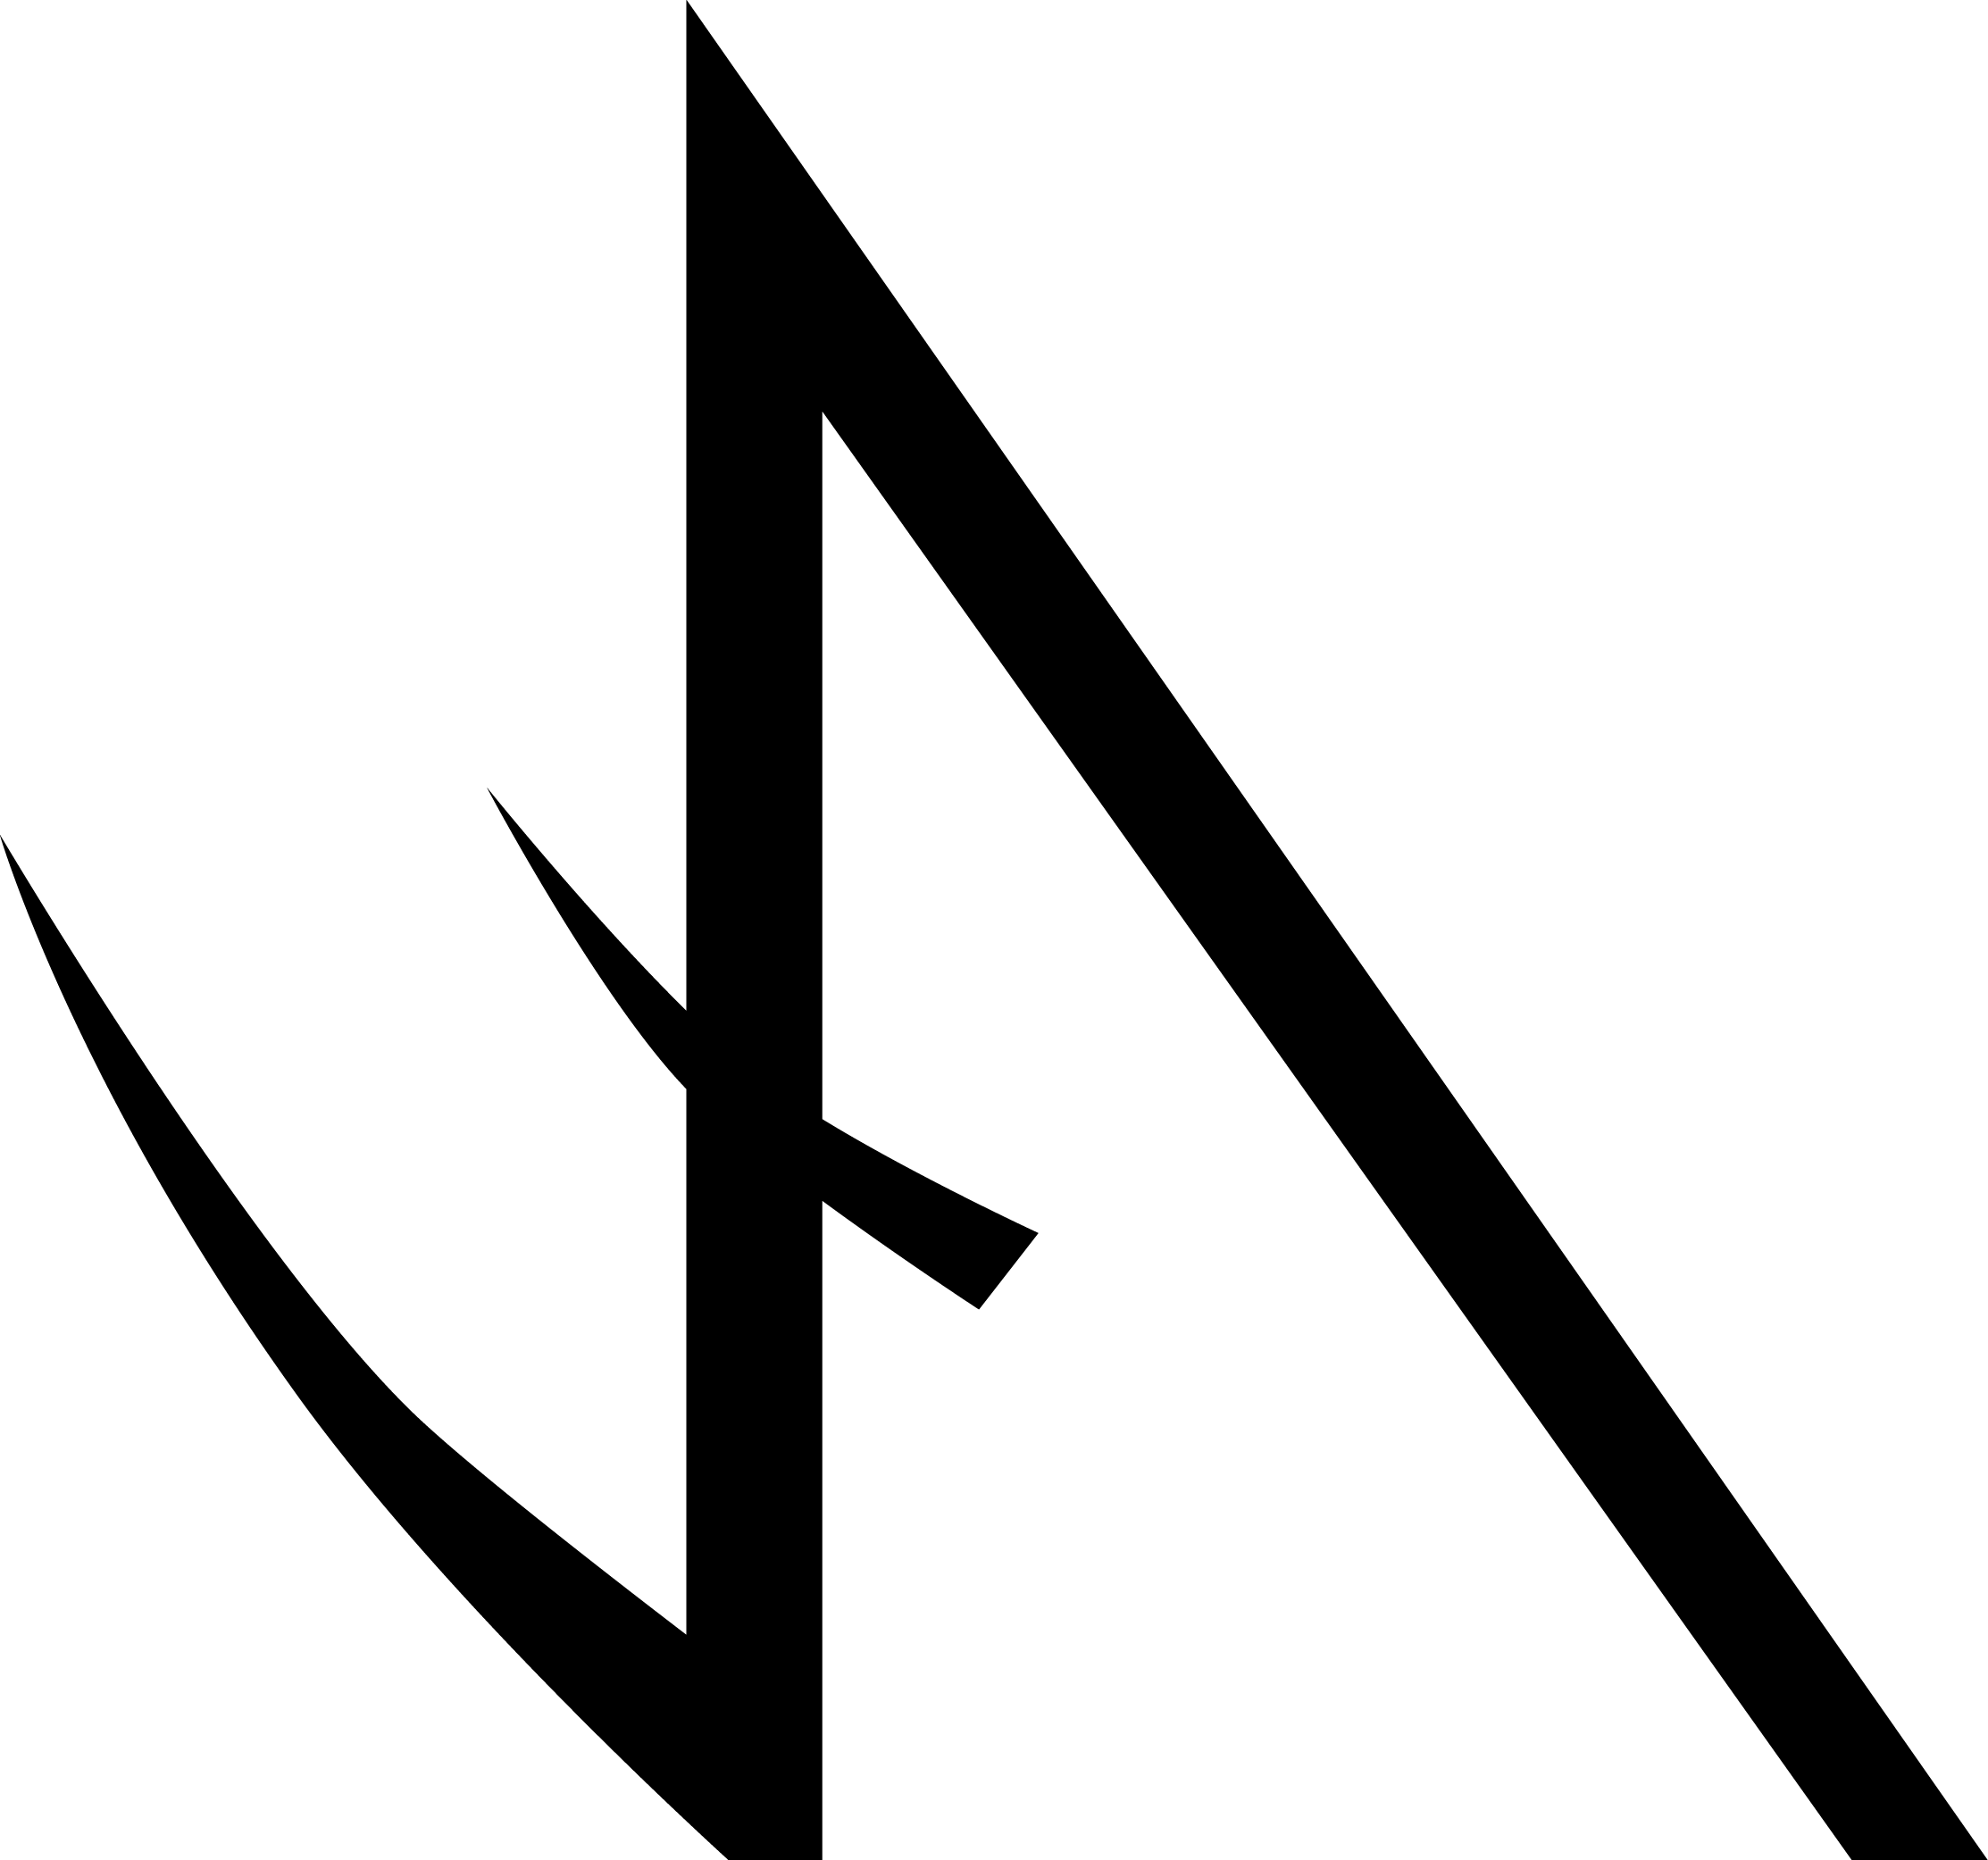
\includegraphics[height=1em]{images/Pewter_(Feruchemy).png}}
A Pewter Misting is called a Thug.\cite{ARS}  Pewter is a physical internal pushing metal.\cite{AL-TB}  Burning Pewter results in the user gaining significant strength, and speed.\cite{ARS}  It also grants a small but significant healing factor,\cite{HoA-CH26} and heightens several internal senses such as proprioception and balance.\cite{TFE-CH5}

Pewter is an exceptionally dangerous metal to burn for long periods\cite{TFE-CH24}\cite{TFE-CH25} as it suppresses some warning senses such as exhaustion and pain.\cite{TFE-CH7}  It is possible for a normal thug to die from Pewter withdrawals after a long period of burning.  A burn such as this is referred to a Pewter drag.\cite{TFE-CH26}\\

A Pewter Ferring is called a Brute.\cite{ARS}  Pewter can be used to store physical strength.  When storing, the Brute is weak and shriveled, but when tapping, a Brute's mussel become physically larger and more powerful.\cite{WoA-CH53} \\

Compounding Pewter would allow for amazing amounts of strength to be stored, however, due to the mussel size increase, only a limited amount can be tapped at any one time without a Brute effectively loosing the ability to move.\cite{Bodybuilder}\\

Pewter Savantism is exceedingly dangerous, and frequently fatal.\cite{WoF}  The benefits would be a massive increase in the potential output of Pewter, particularly in healing factor.cite{AoL-CH17}  However, the downsides may include the inability to heal or move at all when not burning Pewter.\cite{HoA-CH56}  Since Pewter withdrawal after an extended burn can be dangerous all on its own, the effects of a savant running out of Pewter are probably devastating.\cite{WoF}  Due to the dangers, the only confirmed Pewter Savant is Tarson, a koloss-blooded Vanisher.\cite{AoL-CH17}\\

In Hemalurgy, a Pewter spike steals physical Feruchemical abilities.\cite{HE-TB}\\

In Fabrial tech Pewter does the opposite of Tin, and creates an augmenter that enhances the element within,\cite{RoW-E9} notable examples are the heat radiating fabrials\cite{WoK-CH15}, and the one-off inverse painreal which can deliver extreme pain at a touch.\cite{RoW-CH84}  Interestingly, Pewter fabrials consume more Stormlight than other equivalent fabrials made with other metals.\cite{RoW-E9}

\subsection*{
\includegraphics[height=1em]{images/Zinc.png}  Zinc 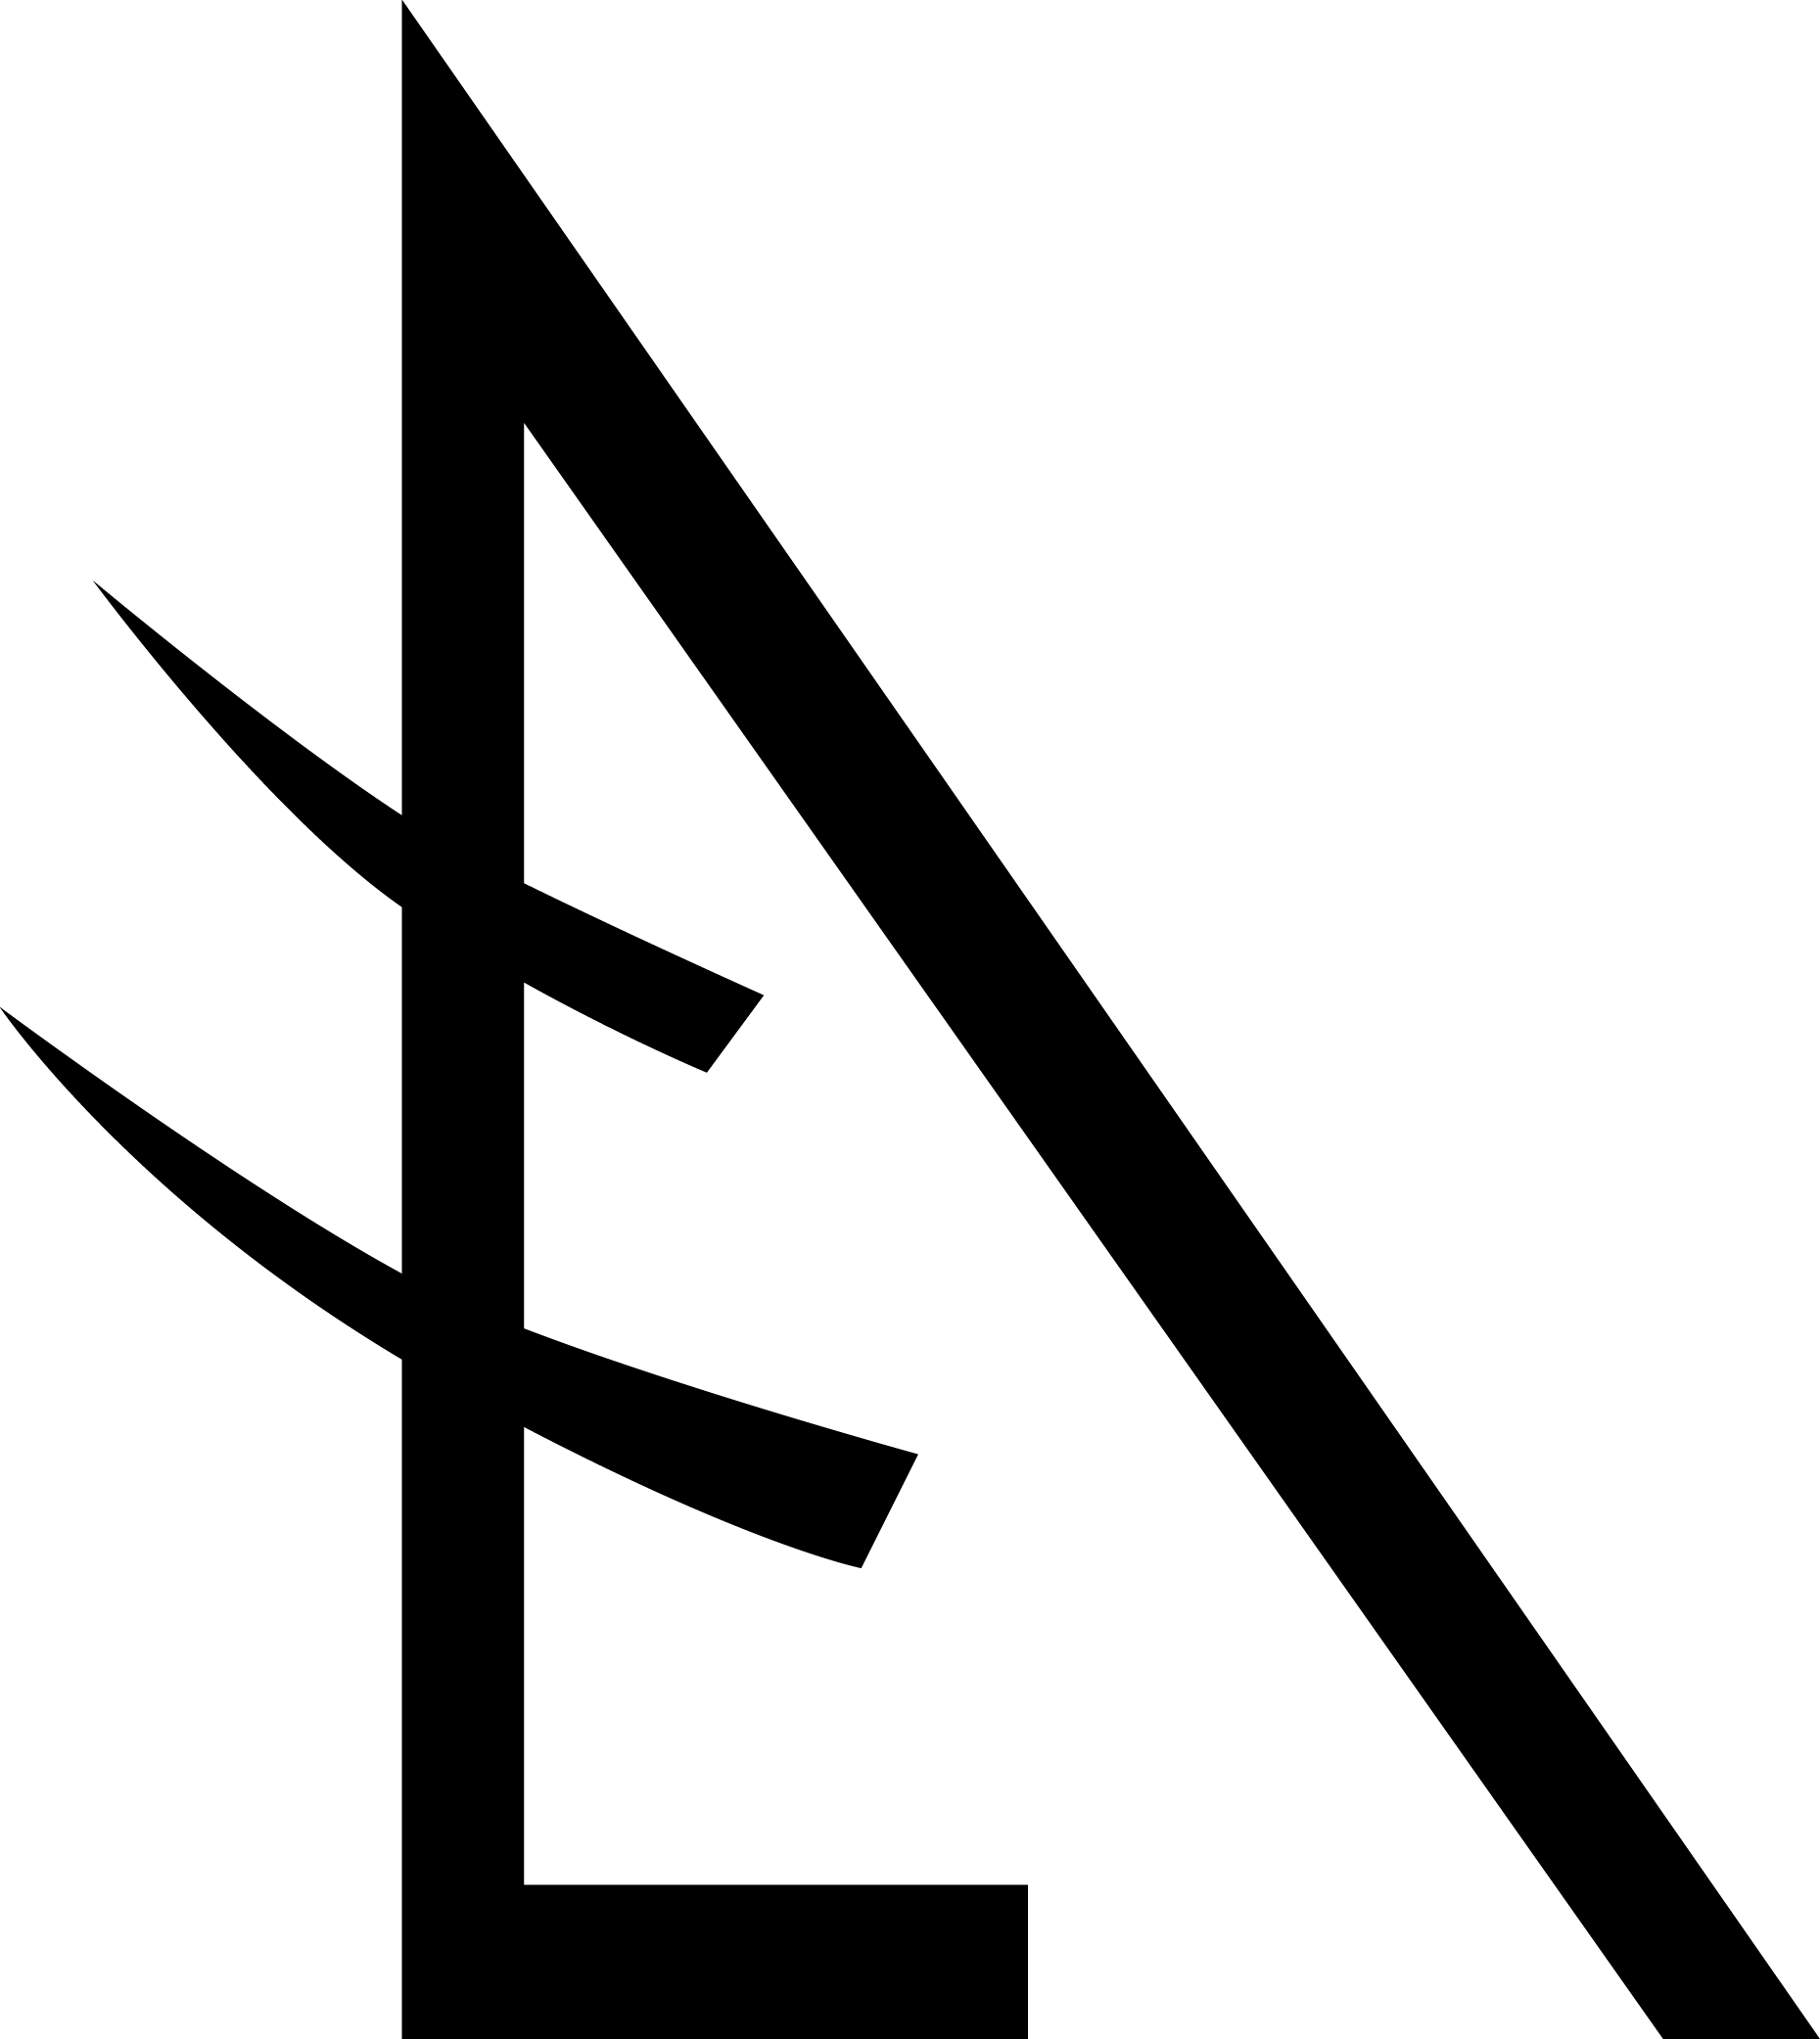
\includegraphics[height=1em]{images/Zinc_(Feruchemy).png}}
A Zinc Misting is called a Rioter.\cite{ARS}  Zinc is a mental external pulling metal.\cite{AL-TB}  A Rioter can ``pull" on the emotions of another person making them stronger.\cite{ARS}  A Rioter can not effect them self.\cite{WoA-CH46}  Except in the case of Hemalurgic constructs,\cite{WoA-CH40}\cite{WoA-CH54} a Rioter can not directly control another person, and can only make them feel a specific way.\cite{TFE-CH4}  The emotional influence can be quite subtle or extremely powerful.\cite{TFE-CH10}

Rioting has a few notable weaknesses, a person can be trained to detect when emotional Allomancy is being used on them,\cite{TFE-CH2} a Bronze Seeker can determine which emotions are being manipulated,\cite{TFE-CH20} and a Copper Smoker is immune while burning.\cite{TFE-CH7}  Additionally the effects of Rioting can not pass through Aluminum, so an Aluminum hat is a viable protection as well.\cite{AoL-CH3}  Interestingly, the prime researcher has also suggested that Shardplate helmets also block emotional Allomancy,\cite{Shardplate} although it is unknown if emotional Allomancy can be used by someone wearing Shardplate themselves.

A powerful Rioter,\cite{WoF} a group of Rioters,\cite{HoA-CH5} or an enhanced Rioter\cite{WoA-CH54} can take control of any Hemalurgic construct\cite{WoA-CH40}\cite{WoA-CH54} with 2\cite{WoA-CH40} or more spikes that isn't already being controlled by a more powerful entity.\cite{HoA-CH3}  It is unknown if a non construct with 2 Hemalurgic spikes are also weak to this effect.  However, the effects of Rioting are more effective against non constructs with any number of spikes.  

Rioting can effect non human animals with some degree of sapience.\cite{riot-animal}\\

A Zinc Ferring is called a Sparker.\cite{ARS}  Zinc is classified a cognitive not mental Feruchemical metal, although the difference seems academic.\cite{FE-TB}  A Sparker can store mental speed.  So by tapping Zinc, a Sparker can get a ``Spark" of genius.\cite{ARS}  Oddly this increased mental speed makes the user hungry,\cite{BoM-CH3} it is possible the energy required to ``overclock" the mind is not stored in the metalmind.\\

Compounding Zinc is extremely potent, as it would allow the user to gain near infinite intelligence.  This effect could meet or exceed the ``Brightest" day where Taravangian laid down the Diagram, an effective prediction of all major events on Roshar for 5 years (including several events that should not be predictable).\cite{WoR}\cite{OB-CH122}  A Zinc compounder could have access to this level of intellect if not higher.  It would likely be possible for a Zinc compounder to create a new Hemalurgic construct.  This is assuming the effects of hunger don't kill the compounder.

It may be the case that ``Mental Speed" and ``Intelligence" are not the same.\cite{MSI-N}  However, this distinction is debated even outside of the scope of Feruchemical Tin.\cite{MSI-P1}\cite{MSI-P2}\cite{MSI-P3}
\\

Zinc Savantism is interesting.  There are no known Zinc Savants,\cite{WoF} however it is quite similar to that of Brass, and all Brass users known are nearly always burning Brass.\cite{WoA-CH11}  This suggests there should be many Zinc and Brass Savants.  Possibly Zinc savantism shows minimal effects on the user as Zinc is an external power.  The effect could be simply a more subtle control of emotion.

An interesting side effect is that it may be possible for a person to become addicted to the effects of emotional Allomancy being used on them, for example a Rioter rioting their happiness.  This could create a savant like effect in a non Allomancer. \\

When used as a Hemalurgic spike, Zinc steals ``Emotional Fortitude."\cite{HE-TB} It is unknown exactly what this does, it is distinct from depression which is linked to determination. \cite{ARS}  Possibly this creates a resistance to Emotional Allomancy.  In Kandra, Zinc spikes form the Blessing of Stability\cite{Bless-stable} which does grant resistance to the control of emotional Allomancy,\cite{WoA-CH54}\cite{WoA-CH40} so this theory has some backing.\\

In Fabrial Tech, Zinc increases the effect of another fabrial.\cite{RoW-E7}

\subsection*{
\includegraphics[height=1em]{images/Brass.png}  Brass 
\includegraphics[height=1em]{images/Brass_(Feruchemy).png}}
A Brass Misting is called a Soother.\cite{ARS}  Brass is a Mental External Pushing metal.\cite{AL-TB}  Allomanticaly, Brass is nearly identical to Zinc, except it suppresses emotions instead of heightening them.\cite{ARS}
According the the prime researcher, it can also be used to suppress a singers ability to hear a rhythm.\cite{soothe-rythem}  This indirectly means a Rioter could make it easier to hear a rhythm, or possibly force a rhythm to be heard.\\

A Brass Ferring is called a Pinnacle.\cite{ARS}  A Pinnacle can store determination, becoming depressed while storing, but being able to become manic by tapping.  Like Zinc, Brass is also classified Cognitive, not mental.\cite{FE-TB}  
The keen eyed among you may notice that this description does not match up with the description as outlined in the books or on the wiki, but does match with that of Electrum.  This is intentional.  The official effect of Brass is storing heat, when questioned why heat was a cognitive ability, the Prime Researcher responded that he had made a mistake.\cite{mistake}  In \textit{Mistborn: The Final Empire}, the effect of Brass is listed as storing heat, however this is incorrect.  The mistake was not caught until long after publishing, and rather than retconing the effect, the prime researcher just swapped them in cannon.  This further reinforces that the Prime researcher can be wrong.\cite{unreliability}  The effect of Brass is really determination, not heat.  As the purpose of this Journal is accuracy, not story consistency, we will encourage the use of Brass and Electrum with their correct effects, not their incorrect but official effects.  Only their Feruchemical effect was swapped, the Allomantic and Hemalurgic effects remain unchanged.\\

Compounding Brass allows for a large amount of manic emotion to be built up and tapped as needed.  This is likely of minimal use other than mental health.  As metalminds are generally keyed, this is of minimal use.  If stored in unkeyed or unsealed metalminds, a Brass compounder should be able to supply a large number of depressed people with an anti-depression aid.\\

Brass Savantism is likely similar to Zinc.  As noted in Zinc, there are oddly few Savants given most users burn most of the time.\cite{WoA-CH11} \\

In Hemalurgy, Brass Steels the Cognitive Feruchemical powers.\cite{HE-TB}\\

In Fabrial Tech, Brass decreases the effect of another fabrial.\cite{RoW-E7} 
\subsection*{
\includegraphics[height=1em]{images/Bronze.png}  Bronze 
\includegraphics[height=1em]{images/Bronze_(Feruchemy).png}}
A Bronze Misting is called a Seeker.\cite{ARS}  Bronze is a mental internal pushing metal. \cite{AL-TB}
A Seeker can ``feel" other Allomancers who are burning metals.\cite{ARS}  The Seeker can feel direction and rough intensity, as determined both by distance and strength of burn.\cite{TFE-CH20}  Each metal has a unique feel, so a trained Seeker can determine which metals are being burned.  An extremely trained Seeker can detect what emotion a Soother or Rioter is influencing. \cite{TFE-CH20}

While generally used for finding active uses of Allomancy, it should be possible for a Seeker to detect any investiture\cite{seek-univeral} including Feruchemy,\cite{seek-FE} Surgebinding (including differentiating surges),\cite{seek-surge} AonDor,\cite{seek-aone} Awakening,\cite{seek-aone} Summoned Shardblades,\cite{seek-shard} active Fabrials,\cite{OB-CH69}\cite{seeker-spren} the Rhythms of Roshar,\cite{seek-rythem} and possibly open Perpendicularitys\cite{HoA-CH37}.  While not directly confirmed, a Seeker could also probably detect a working Sandmaster and a coming Highstorm.  Shards can also create fake pulses to emulate anything a Seeker can detect,\cite{HoA-CH37}\cite{HoA-CH38} these can be targeted at a specific Seeker.\cite{HoA-CH38}

This feeling manifests as a specific ``rhythm" of pulses,\cite{TFE-CH20} similar to the Rhythms of Roshar (which a Seeker could hear)\cite{listner-seeker}.\cite{seek-rythem}  It is possible that the ``tone" of the pulses matches the shard responsible for the Investiture.\cite{shard-lengh}\cite{pure-tone}  So Allomantic pulses are heard in Preservation's tone.

Generally Seekers have difficulty detecting internal investiture,\cite{seek-FE} and there are no instances of Feruchemy being detected by a Seeker. 

A powerful Seeker can pierce a Copper cloud (see Copper).\cite{TFE-CH31}
A Seeker likely can not pierce Aluminum, such as an Allomancer in an Aluminum box.\cite{OB-CH81}  This is not the most relevant for Allomancy as most abilities would be relatively useless in such a box, however compounders could safely compound within such a box without being detected, and fabrials can be used within one without being detected.\\

A Bronze Ferring is called a Sentry.\cite{ARS}  Similar to Brass and Zinc, the Feruchemical classification is Cognitive, not mental.\cite{FE-TB}  Filling a Bronze metalmind makes its user drowsy.\cite{ARS}  A Sentry can decide how long to sleep, and fill a Bronze mind while sleeping. Bronze is the only Feruchemical ability that can be used while sleeping.\cite{WoA-CH57} This sleep likely does count as regular sleep.\cite{TFE-CH22}  This wakefulness can be taped to keep the user awake and alert indefinitely.  A Sentry can also store ``wakefulness" from chemical stimulants such as caffeine, however tapping it would then feel like using the stimulant.\cite{BZ-FE-Chem}\\

Compounding Bronze is extremely useful, in theory it can be used to stay awake forever with no negative effects, and constantly feel alert and awake as if well rested.\cite{bronze-comp}  It should be noted at this point that compounding becomes decreasingly effective over time as more of the compounded attribute is used, so it is possible that the longer such a compounded stayed awake, the more frequently they would need to compound to do so.\cite{AoL-CH13}\cite{TFE-CH38}  It is unknown if a single nights rest would reset the compounding requirement, and sudden withdrawal from an extended Bronze compounded may be enough kill the compounder.\\

A Bronze Savant would have an expanded range and increased Copper piercing power.\cite{WoF}\cite{savant-pierce}\cite{seeker-savant-compound}  They would also likely be able to determine more investiture sources, such as being able to distinguish between Allomancy and Compounding.\cite{seeker-savant-compound}
The downsides of Bronze savantism are minimal, and many Seekers have likely become savants without knowing.\cite{WoF}\cite{savant-pierce}\\

A Bronze Hemalurgic spike steals Mental Allomantic Powers.\cite{HE-TB}\\

In Fabrial Tech, Bronze allows for the creation of remote triggers,\cite{RoW-E8}  Such as a fabrial that warns if anyone new approaches within a specified range.\cite{WoR-I4}
\subsection*{
\includegraphics[height=1em]{images/Copper.png}  Copper 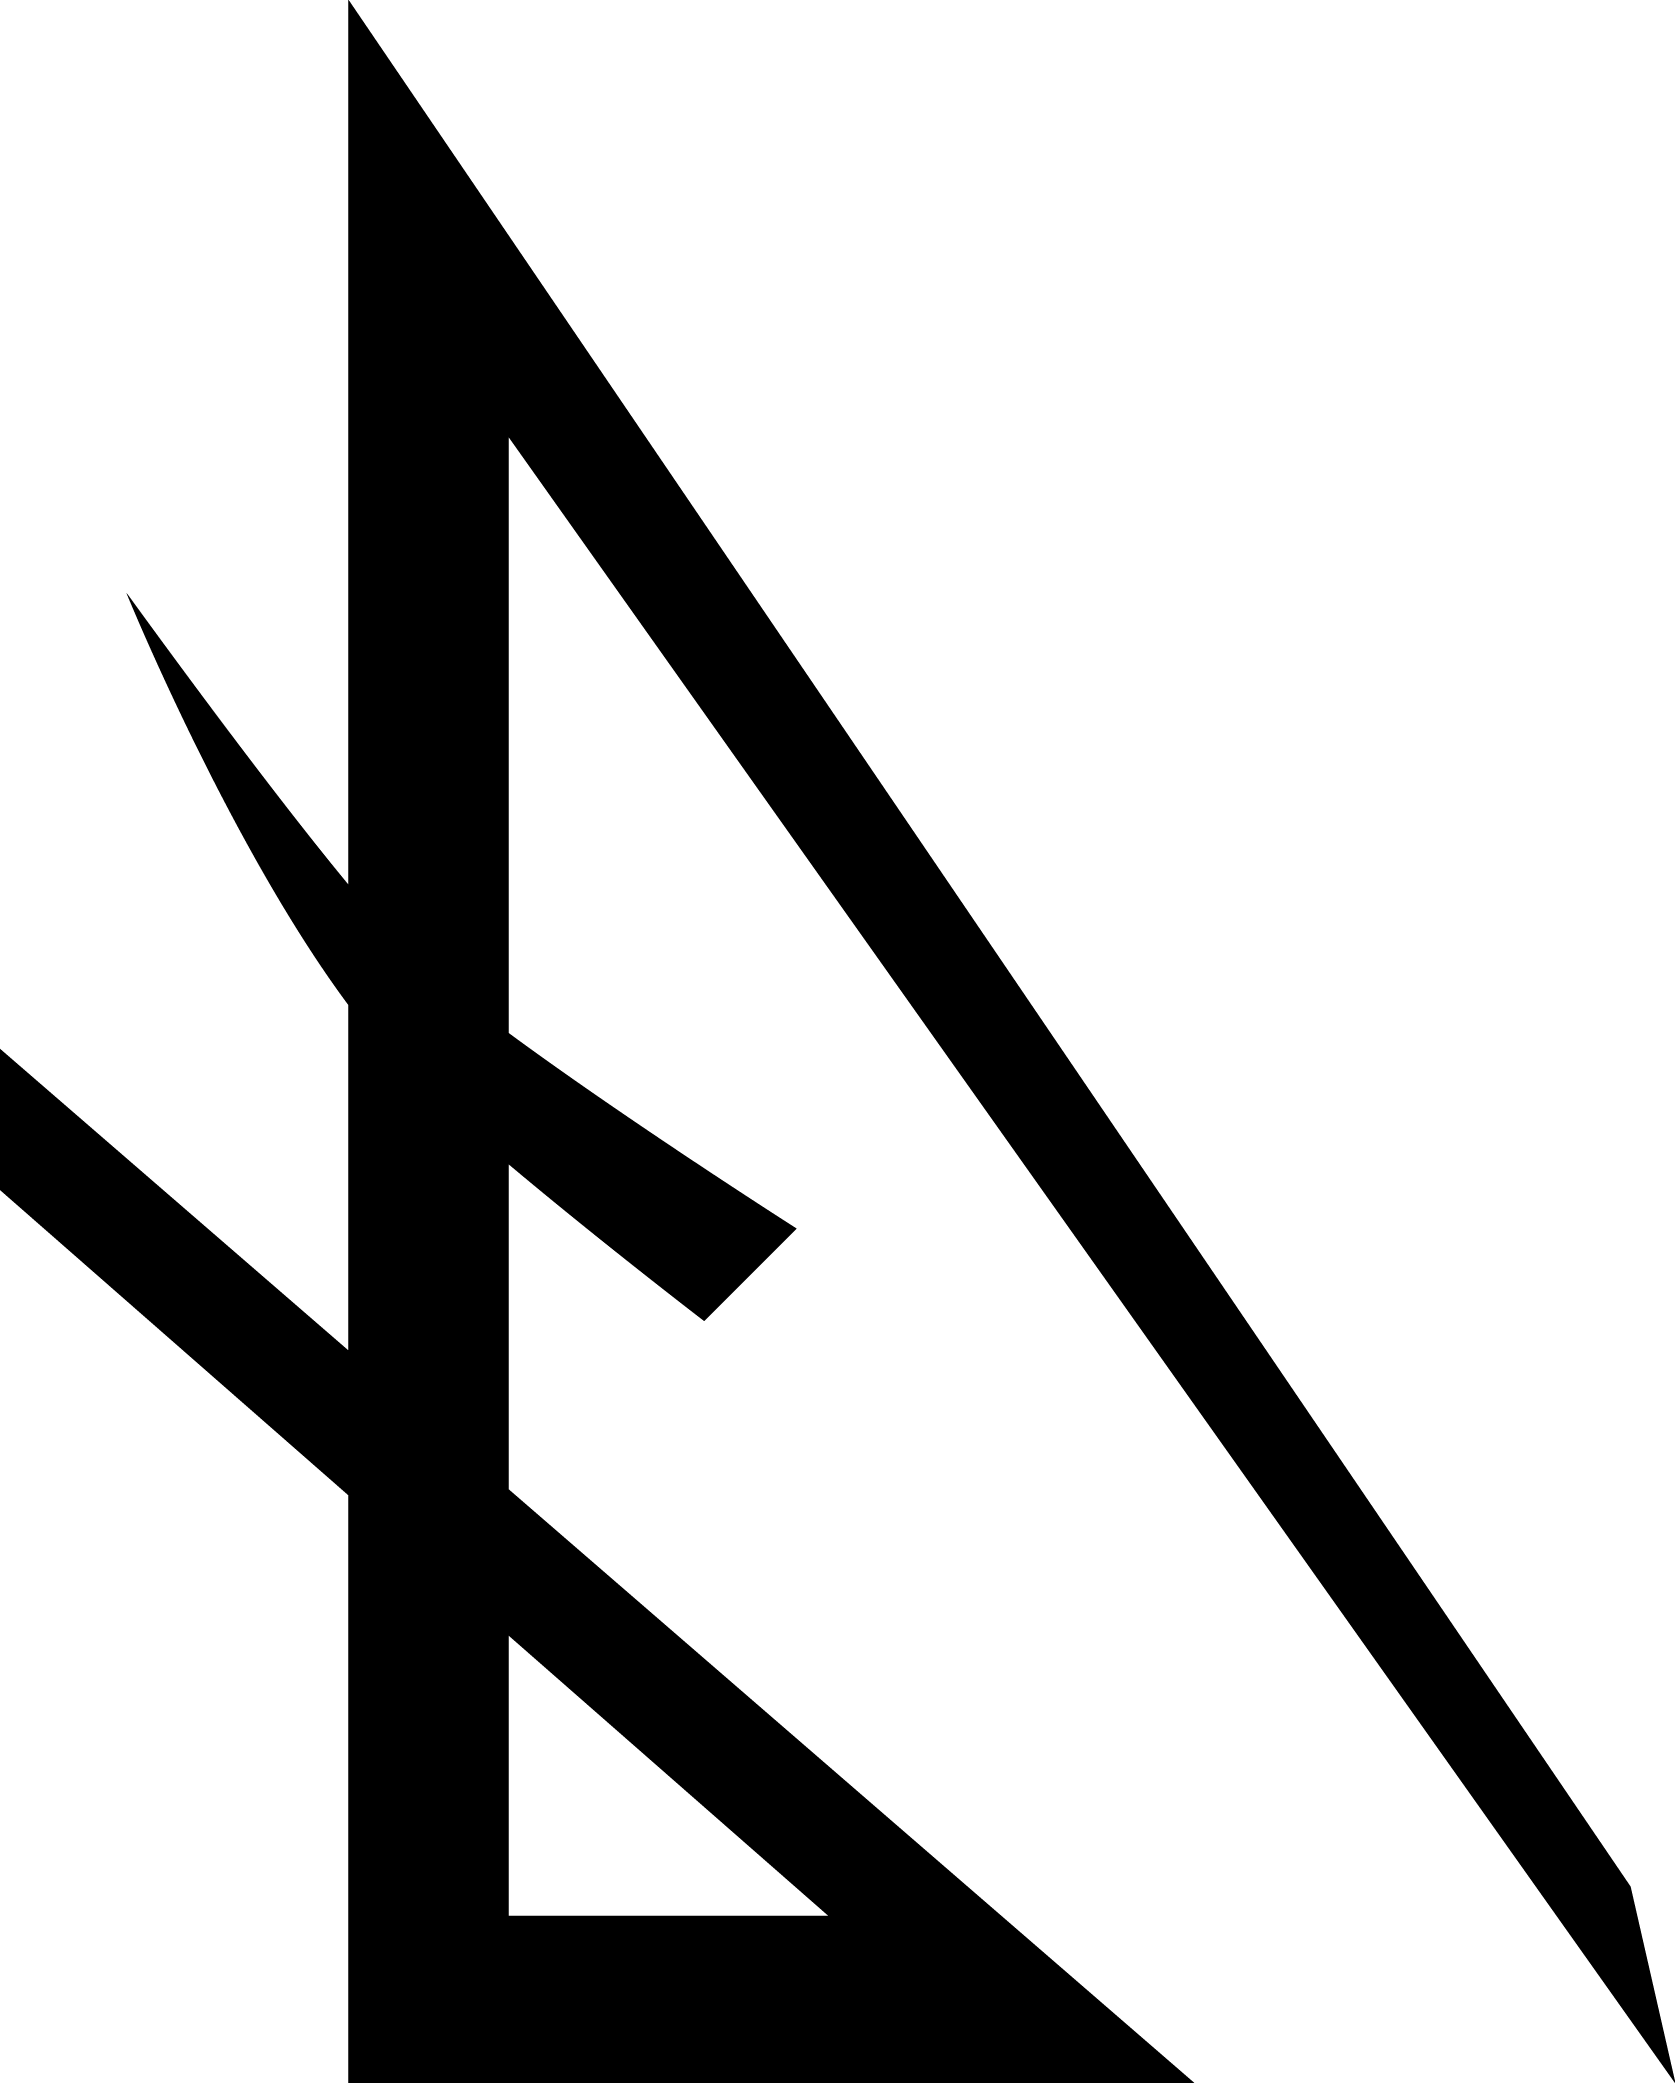
\includegraphics[height=1em]{images/Copper_(Feruchemy).png}}
A Copper Misting is called a Smoker.\cite{ARS}  Copper is a mental internal pulling metal.\cite{AL-TB}  This exact designation is mostly based on inference.  A Smoker can burn Copper to create a ``Copper cloud" around them, this cloud hides all investiture use within its radius from Seekers.\cite{ARS}  Because of this, its Bronze pulse signature was not publicly known for some time, and its placement was based on that of its alloy Bronze.\cite{TFE-CH20}\cite{TFE-CH7}
It is possible for a Copper cloud to be pierced by a powerful Seeker,\cite{TFE-CH31} but it is also possible for a Smoker to become more powerful to hide from such a Seeker.\cite{TFE-CH31}  These power boosts can come from various sources including skill, Hemalurgy, and enhancement Allomancy, but if equal in power, Copper wins.  A Seeker must be significantly more powerful than a Smoker to pierce the cloud.\cite{TFE-CH31}

A Smoker can also hide other investiture sources and hide from other detection sources.\cite{seeker-spren}  For example, a Smoker could likely approach a warning fabrial without triggering it.  This would also stop Awakeners lifesense/aura recognition.\cite{life-block}  Oddly the prime researcher has stated Copper clouds can affect spren,\cite{copper-spren} and prevent singers attuning a Rhythm.\cite{rythm-block}

A Smoker's mind is protected from emotional Allomancy while burning.\cite{TFE-CH7}  It may be possible but difficult to extend this in a bubble.\cite{emo-cloud}

It may be possible in a similar way to prevent a Lurcher or Coinshot from using a piece of metal as an anchor.  However this is unknown.  If possible, it may also be possible to block any use of investiture such as the summoning of a Shardblade.\cite{rythm-block}\cite{emo-cloud}\cite{ARS}

It is unknown if a Smoker with Hemalurgic spikes is protected from shard influence while burning.\\

A Copper Ferring is called an Archivist.\cite{ARS}  Similar to Brass, Zinc, and Bronze, the Feruchemical classification is Cognitive, not mental.\cite{FE-TB} 

A Copper metalmind can be used to store memories without them decaying.  A memory stored in this way is forgotten by the Archivist.\cite{ARS}  Memories stored in this fashion are vulnerable to the manipulation of a shard.\cite{WoA-EP}  An Archivist can access individual memories in a Copper metalmind,\cite{copper-ia} and frequently create memory indexes\cite{WoA-CH4} to help locate them, similar to a hard drive.
Memories do not decay within a metalmind, but will decay when accessed since the memory is moved to the Archivists mind temporarily.\cite{WoA-CH15}

Only memories can be stored, not generic neuron patterns such as skills or ``muscle" memories.\cite{copper-no-mm}\\

Copper compounding is an odd effect.  Memories are non-fungible, whereas all other stored attributes are fungible.  Compounding other attributes is as simple as creating more of them, but what this would do to a memory is not clear.  It is our opinion that compounding Copper would allow a memory to be copied.  This would allow an Archivist to store a memory, then compound that memory into 2 copies, one to store in a metalmind, and one to remember in their actual mind.\\
 
A Copper Savant likely has an increased range and Bronze resistance.\cite{savant-pierce}  As most Smokers leave their copper on continuously it is likely that nearly ALL smokers are Savants,\cite{WoF} this goes some way to explaining how NO regular Seeker has pierced a copper cloud in hundreds of years.\cite{TFE-CH31}

A Copper Hemalurgic spike can steal mental fortitude, memory, and intelligence.\cite{HE-TB}\\

Copper may have a use in Fabrial Tech, but it is unknown what.  It may invert a Bronze detector, or possibly hide a Fabrial from being detected.

\subsection*{
\includegraphics[height=1em]{images/Aluminum.png}  Aluminum 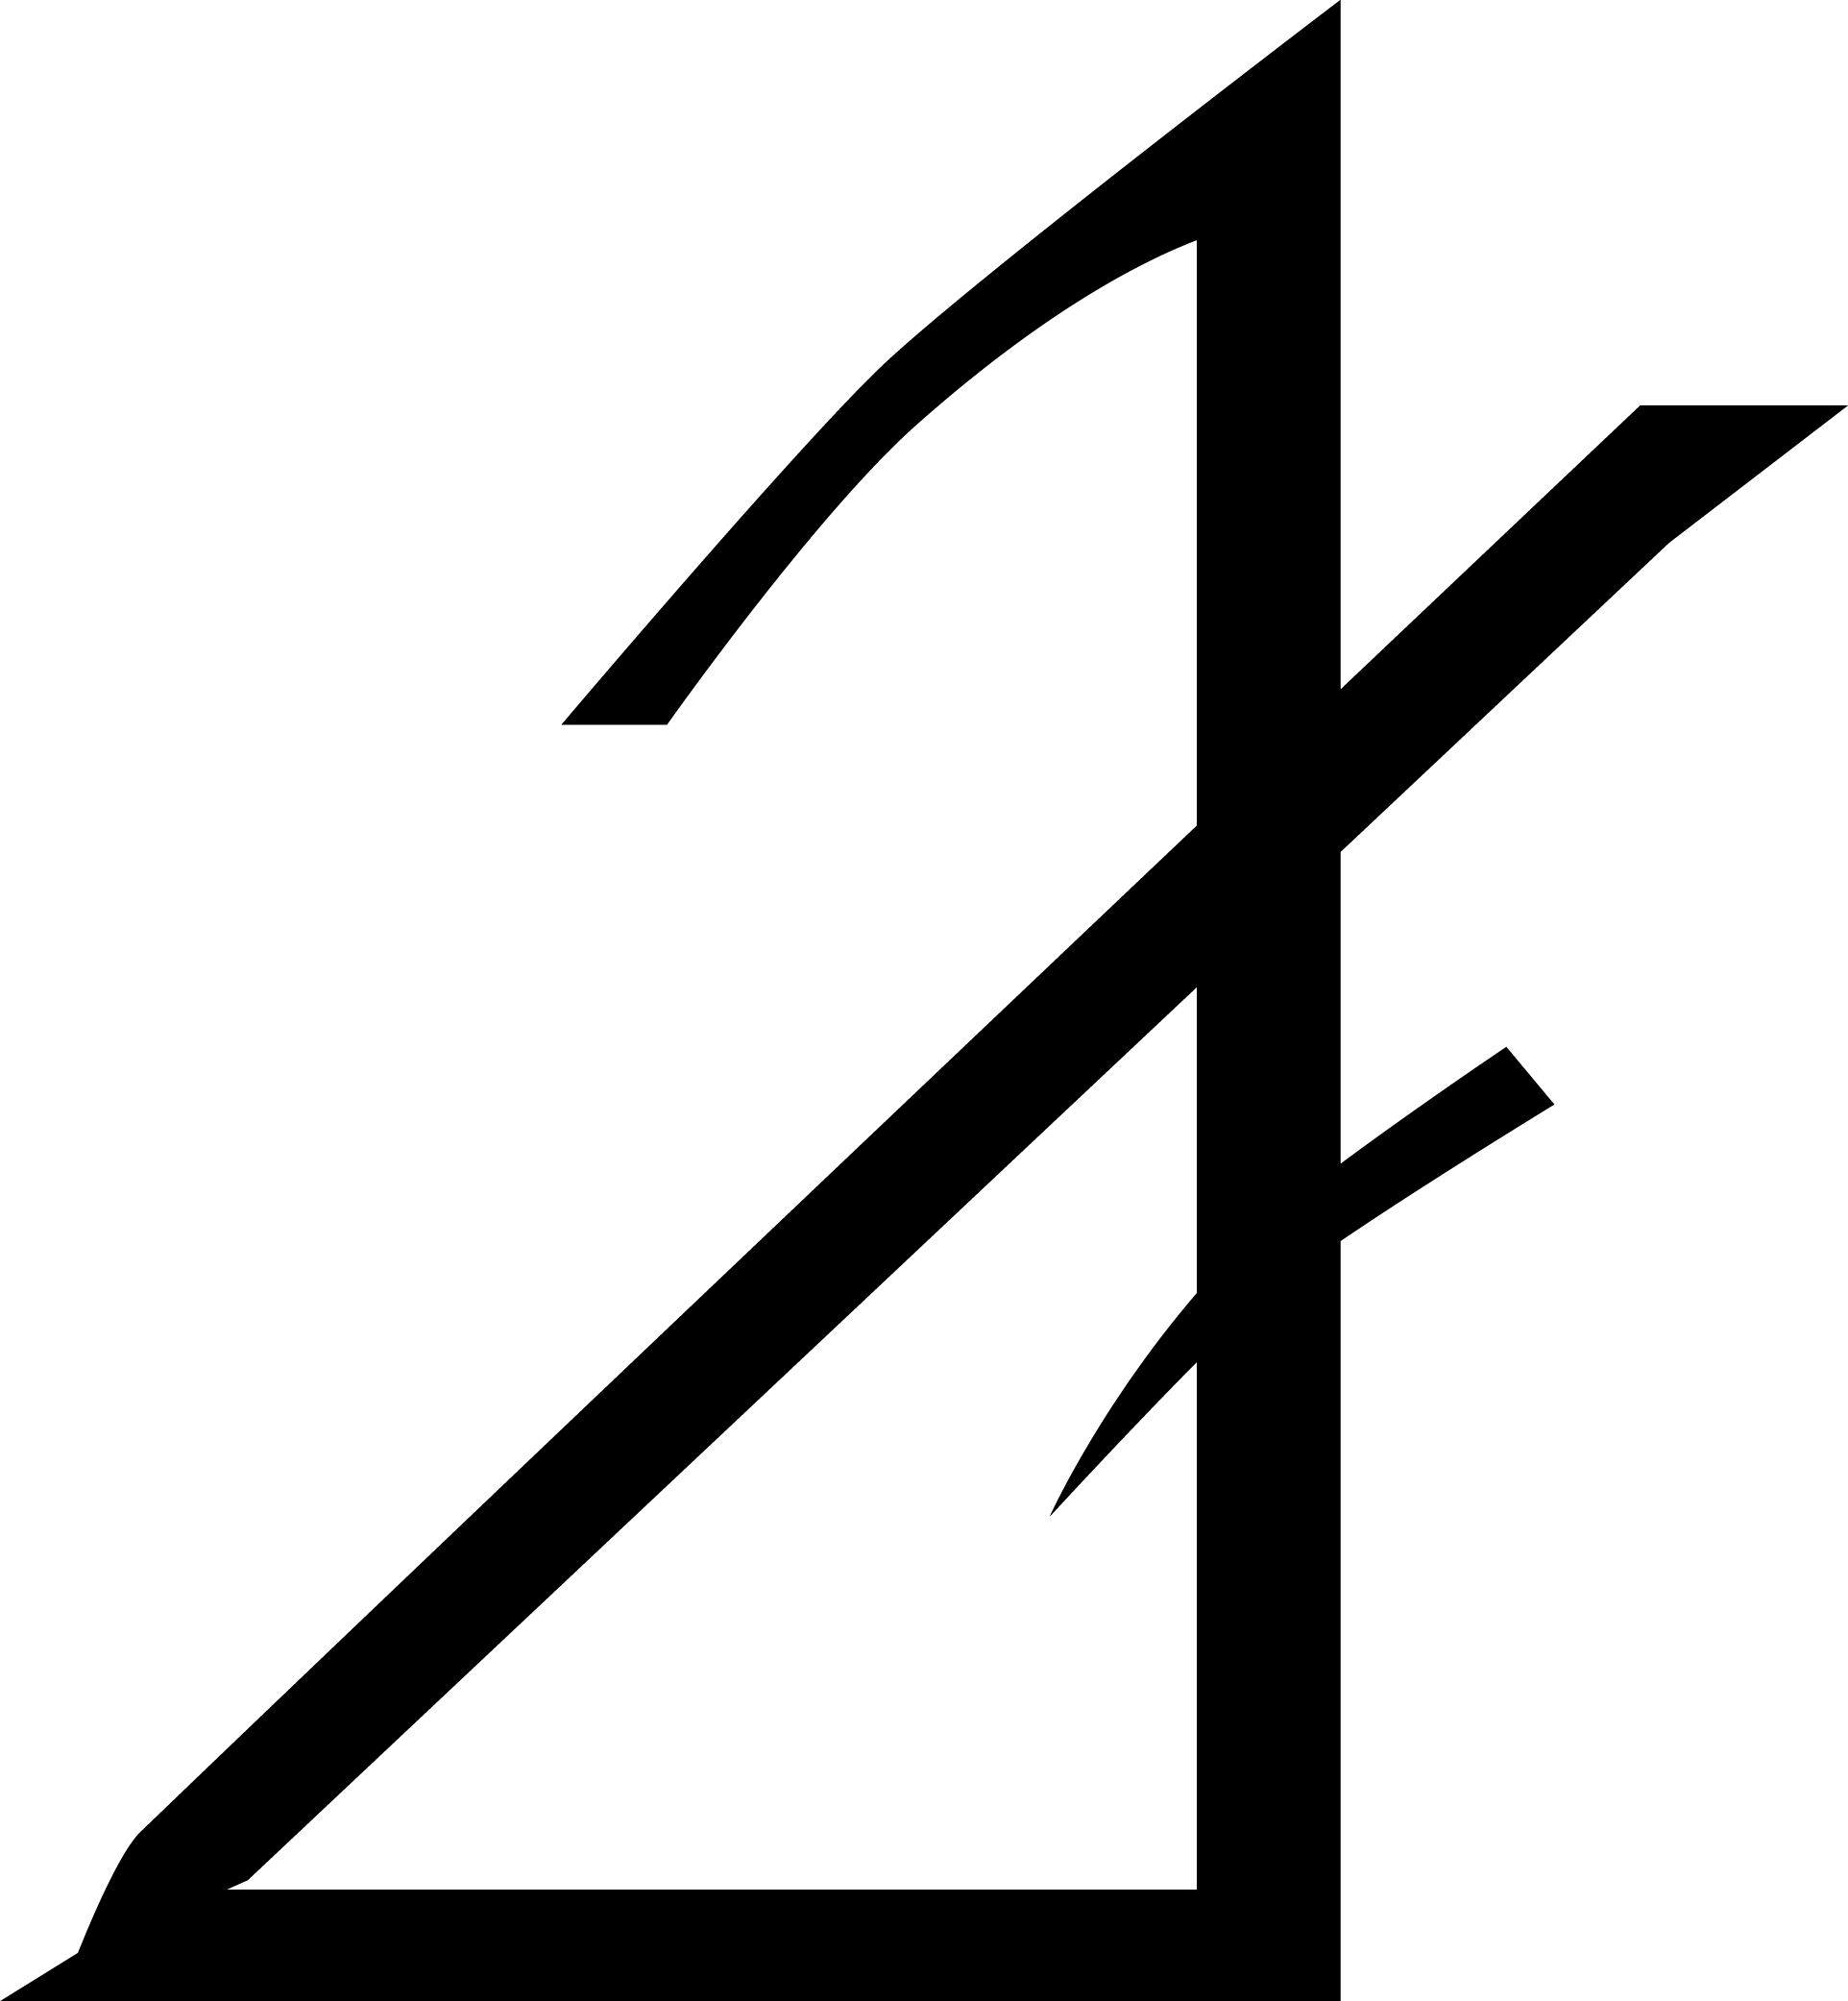
\includegraphics[height=1em]{images/Aluminum_(Feruchemy).png}}
Aluminum (also called Ralkalest\cite{RoW-CH37}) is a particularly noteworthy metal as it is nearly immune to all investiture.\cite{al-universal}  The only know exceptions are Feruchemical,\cite{FE-TB} and Hemalurgy,\cite{HE-TB} in all other contexts (save Allomantic burning\cite{AL-TB}) Aluminum is immutable.  It can not be pushed by a Coinshot, nor pulled by a Lurcher,\cite{ARS} and does not even have a metal line.\cite{BoM-CH6}  It does not cast an Atium* shadow.\cite{al-atium} An Aluminum hat passively protects is wearer from Brass, Zinc,\cite{AoL-CH3} and shards.\cite{al-shard}  An Aluminum box blocks detection void spren\cite{RoW-CH81} and presumably Seekers.  It can not be Soulcast\cite{al-cast} or Forged\cite{al-forged} into something else (although it can be created by Soulcasting\cite{WoR-CH48}).  It can not be magically cut by a Shardblade\cite{RoW-E17} (although a thin sheet could still be ripped by one\cite{RoW-shardblade-wob}), and can effectively contain Nightblood\cite{al-night}.  No form of Surgebinding\cite{RoW-E17}\cite{al-surge} or Voidbinding can effect it or move through it.\cite{RoW-CH37}  If made into a non-Hemalurgic spike, it will block all magical healing factors until removed.\cite{al-hf}  It can not be Awakened,\cite{al-awake} and it will block an Awakeners life sense.\cite{seeker-spren}  In short, it is a hard counter to all forms of investiture, full stop, however it does not actively absorb investiture,\cite{al-awake} it just blocks it.  A bottle made from Aluminum would even be capable of removing invested liquid from a perpendicularity for later use.\cite{al-fluid}\\

An Aluminum Misting is called an Aluminum Gnat.\cite{ARS}  Aluminum is a internal pulling enhancement metal.\cite{AL-TB}  There are only 2 effects of burning Aluminum, first the burner emits Allomantic pulses that can be detected by a Seeker (presumably),\cite{TFE-CH36} and second, all other ingested metal reserves are erased.\cite{ARS}  As such, there is almost no effect of burning Aluminum as a Misting.  This is the only known way to alter the form of Aluminum as it is burned away by the Allomancer.  Burning aluminum would almost certainly purge the body of all other invested fuels such as Stormlight or BioChromatic breaths.  It may be possible that Aluminum only suppresses BioChromatic breaths rather than destroying them, but the only person known to have both Allomantic Aluminum and Breaths is Hoid.\cite{SH-PT2-CH1}\cite{hoid-burn}\cite{WoR-CH45}\cite{WoR-CH59} Burning Aluminum would repair the withering damage dealt by a Threnodite Shade.\cite{gl-shade} This MAY grant the person burning it immunity to other investitures as well.  This is unknown, but given the nature of Aluminum it is likely.\\

An Aluminum Ferring is called a Trueself.\cite{ARS}  Feruchemical Aluminum is a Spiritual metal.\cite{FE-TB}  A Trueself can create an Aluminum metalmind, this is one of only 2 known ways of changing Aluminum into something else.  The Trueself can store and retrieve Identity.\cite{ARS}  The effects of this are not entirely known, but it has a large number of ramifications, most notably  Metalminds are keyed to Identity.  If a Feruchemist capable of storing multiple attributes (either by being a Full Feruchemist or by gaining access to a second through a method such as Hemalurgy), then storing Identity while creating another metalmind at the same time will result in the second metalmind being created WITHOUT an Identity lock on it.  As such, anyone who can tap that attribute can use that metalmind.\cite{BoM-CH3}  It is unknown if the metalmind can be refilled by anyone without keying it.  In a similar fashion a Trueself with BioChromatic breaths could Awaken an item unkeyed so that anyone could retrieve the breaths.\cite{unkeyed-awake}

If a Ferring created an unkeyed Identity metalmind, a person tapping it could then tap any metalminds keyed to that Ferring.\cite{HE-Fe-access}

Identity also seems to have an effect on the regional accent of a person\cite{identy-accent}, by storing Identity, and tapping Connection,\cite{OB-CH65}\cite{BoM-CH22} a person can speak the local language without an accent.\cite{identy-accent}\\

Compounding Aluminum would create more Identity.  What this would do is unclear as most of the uses for Aluminum Feruchemy involve ``blanking" identity by storing it, not making more of it.  \\

The effect of Aluminum savantism is unknown.  Officially they can ``cleanse their spirit of unwanted investiture effects".\cite{al-savant}  What these effects ARE however is unknown. \\

The Hemalurgic use of Aluminum is... odd.  An Aluminum spike will remove all investiture based abilities from its host.\cite{HE-TB}  As an Aluminum bullet does not do this, it implies the Aluminum spike needs to be made into a Hemalurgic spike by spiking another person before it becomes active, especially since a victim is usually killed during the creation of a spike making their lack of abilities rather irrelevant.  Such a spike could be used as an effective (if inhumane) method to restrain a powerful investiture user (such as a Mistborn, Elantrian, etc) for an extended period.\\  

In Fabrial Tech, Aluminum has a unique use.  It blocks other effects.  This has been used with conjoined fabrials to limit the conjoining to a single axis,\cite{RoW-CH19} and can theoretically be used to make a directional attractor fabrial or similar.  This appears to be Aluminum base investiture blocking effect, and not a unique effect to fabrials.

\subsection*{\includegraphics[height=1em]{images/Duralumin.png}  Duralumin \includegraphics[height=1em]{images/Duralumin_(Feruchemy).png}}
A Duralumin Misting is called a Duralumin Gnat.\cite{ARS}  Duralumin is a internal pushing enhancement metal.\cite{AL-TB}  Duralumin only has an effect when burning other metals.  The effect of burning Duralumin while burning another metal is extreme. The entirety of a persons metal reserve in that metal is instantly burned at max power and is immediately used.\cite{ARS}   For example, a Mistborn Soothing someone with a Duralumin fueled surge can completely blank their emotions for a moment.\cite{WoA-ch27}  Duralumin is dangerous to burn as not only can the sheer power released can be difficult to control,\cite{WoA-CH11} but also because all reserves of the metal are now depleted.\cite{WoA-CH38}  Duralumin Iron Tin and Steel are only safe when used in combination with Duralumin Pewter.\cite{WoA-CH11}

A weak Allomancer burning Duralumin and Zinc or Brass can take control of a Hemalurgic construct.\cite{WoA-CH40}\cite{WoA-CH54}

Duralumin would also effect other investiture systems in a similar manner.\cite{dl-universal}\\

A Duralumin Ferring is called a Connector.\cite{ARS}  Duralumin is a Spiritual metal.\cite{FE-TB}  As the name suggests, Duralumin is used to store Connection.  Connection includes awareness of other people, friendship, and bonds.\cite{ARS}  Storing connection does not allow an individual to bypass planetary investiture connection.\cite{con-travel}
The Nahel bond can be stored in such a way, but this is probably a bad idea.\cite{con-nahel}

Duralumin is also possibly a required ingredient in an unsealed metalmind.  The idea being, that it acts to connect the wearer to the Nicrosil reserve.

Tapping connection allows for many things.  Firstly, tapping connection will connect the Connector to the geographic area and will allow them to speak the local language,\cite{BoM-CH22} all be it with an accent.  This would allow a connector to interpret the Rhythms of Roshar.\cite{con-rhy}  Secondly, any geographic restrictions on investiture, such as Elantrian Aons, can be overridden by retrieving the required connection from a metalmind.\cite{con-lock}  \\

Compounding Connection would allow for infinite connection.  Apart from the obvious of allowing for the creation of unkeyed translation metalminds,\cite{BoM-CH22} this connection can also be used directly to control Hemalurgic constructs.\cite{con-con}
It is likely a Connection compounder would be similar to a Bondsmith in some respects.\cite{RoW-CH111}\\

Compounding while using Duralumin to enhance it would be dangerous.  The same amount of power would be created all at once making it difficult to control and store.  As such, we would not recommend using Duralumin to boost compounding in most cases.\cite{dl-comp}\\

The effect of Duralumin Savantism are completely unknown.  Duralumin does not increase available power, it only makes it all available immediately.  If one were to theorize, it may be possible a Duralumin savant could extend the surge time?  This seems unlikely and there are no recorded Duralumin savants to reference.\\

The Hemalurgic use of Duralumin is to steal Connection and Identity.\cite{dl-comp}  Possibly this is related to the ability to force another to take the weakness from a Hemalurgic spike.\cite{BoM-CH27}\\

There is no known use for Duralumin in Fabrial tech.  It may be undiscovered on Roshar.
\subsection*{\includegraphics[height=1em]{images/Chromium.png}  Chromium \includegraphics[height=1em]{images/Chromium_(Feruchemy).png}}
A Chromium Misting is known as a Leacher.\cite{ARS}  Chromium is a external pulling enhancement metal.\cite{AL-TB} A Leacher can erase the metal reserves of another person by touching them.\cite{ARS}  This is similar to burning Aluminum, but in another person.  A Leacher can drain other investitures as well such as Stormlight\cite{leech-storm} or BioChromatic breaths.\cite{leech-breath}  A Leacher can effectively render any investiture system unavailable including Feruchemical tapping,\cite{leech-fe} Shardblades,\cite{leech-blade} and Fabrials,\cite{leech-disarm} but it can not Leach the ability its self.  This does not grant the investiture to the Leacher.\cite{leech-disarm}\\

A Chromium Ferring is called a Spinner,\cite{ARS} a Spinner can store Fortune, becoming unlucky as they fill, and lucky as they tap.\cite{ARS}  Feruchemical Chromium is a Spiritual metal.\cite{FE-TB}\\

Compounding Chromium is an extremely scary prospect.  Odium has implied fortune can be used to see the future.\cite{OB-CH122}  It is highly likely that compounding fortune would allow a compounded to see the lines of fate around them and predict the future.\cite{atium-forutne}  This may be a byproduct however, and not the complete effect.  To pull an example from fiction, we suspect a Chromium compounder would be similar to Mobius boosted Nick Campbell from Drew Hayes' Super Powereds.\cite{nick-cambll}

Another probable result of tapping or compounding fortune is that shards can no longer predict the actions of the Spinner.  This has only been indirectly seen when Odium shows how far into the future he can predict, and the only spot hidden from him surrounds a individual with future sight.\cite{RoW-I6}\\

It is unknown what a Chromium savant would be like, possibly it would allow the Leacher to leach at a small range rather than just touch. A fortune compounding savant is likely extremely dangerous.\\

The Hemalurgic use of Chromium is not entirely known, existing sources list it merely as ``probably steals destiny."\cite{HE-TB}  Whether or not this is the actual effect of Chromium is unknown, and what ``stealing destiny" would even do is also unknown.  \\

It is not known if Chromium has a use in fabrial tech, however, it has been shown it is possible to make a fabrial that suppress radiant\cite{RoW-CH9} or void\cite{RoW-CH39} based powers in an area.  Given the Allomantic effect of Chromium, it is not unreasonably to guess that it may be involved in the construction of these fabrials.
\subsection*{\includegraphics[height=1em]{images/Nicrosil.png}  Nicrosil \includegraphics[height=1em]{images/Nicrosil_(Feruchemy).png}}
A Nicrosil Misting is called a Nicroburst.\cite{ARS}  Nicrosil is a external pushing enhancement metal.\cite{AL-TB}  Nicrosil has almost exactly the same Allomantic effect as Duralumin, except the effect is in another person being touched by a Nicroburster instead of in the Nicroburster them-self.\cite{ARS}\\

A Nicrosil Ferring is called a Soulbearer.\cite{ARS}  Feruchemical Nicrosil is a Spiritual metal.\cite{FE-TB}  A Soulbearer can store investiture in a metalmind.\cite{ARS}  The exact effect is complicated and possibly 2 fold.  This appears to store not only investiture, but also the ability to use it.  If a full Feruchemist created an unkeyed Nicrosil metalmind, they could store their ability to use, say, Copper metalminds in the Nicrosil metalmind.  Another Ferring who is a Soulbearer could then tap that metalmind and temporarily gain the ability to use Copper metalminds.  This can be used to store the ability to use other investiture systems if the Soulbearer can use them.  This includes Feruchemy,\cite{BoM-CH21} Allomancy,\cite{BoM-CH28} Stormlight surges,\cite{nic-universal} Divine breaths, \cite{nic-universal}Biochromatic breaths,\cite{PvAvI} and possibly Sandmastery.  
Interestingly, storing investiture also hides a Soulbearer form an Awakener with lifesense.\cite{inv-hid}  It should be noted that all individuals born in the Cosmere have a small amount of innate investiture making them slightly more resilient than Earth Humans,\cite{PvAvI} so there is always an amount of investiture that CAN be stored.

Nicrosil is a key component in an unsealed metalmind as it stores the ability to use the other metals in the metalmind.\cite{BoM-CH21}  The exact composition of an unsealed metalmind is not yet known.\\

Compounding Nicrosil is one of the most useful things to do, as it allows the creation of more ability.  Consider the most powerful metalmind known, the Bands of Mourning.  This unsealed metalmind contains the ability to use all 16 Feruchemical and Allomantic base metals,\cite{BoM-CH28} but since it is a metalmind, its power is limited and will run out.\cite{TFE-CH22}  EXCEPT for Nicrosil compounding which the Bands also transfer the ability to do.  Someone compounding Nicrosil with the Bands of Mourning could refill or even copy them (assuming they know how to make an unsealed metalmind).  Nicrosil compounding logically leads to the commodification of investiture.  With Nicrosil compounders, access to an investiture system could be as simple as purchasing an unsealed metalmind with that system.  As Nicrosil compounders are only limited by the availability of Nicrosil, so too would access to investiture systems become limited only by Nicrosil. \\

Similar to Duralumin, and Chromium, the effects of Nicrosil savantism are unknown and difficult to speculate about, although they are likely a hybrid of the two.\\

In Hemalurgic a Nicrosil spike steals Investiture abilities,\cite{HE-TB} unlike in Feruchemy this is specifically the power its self, not the ability to use the power.\cite{PvAvI}  Otherwise, this would render spikes such as Steel obsolete.  This can be used to steal BioChroma.\cite{PvAvI}\\

There is no known use for Nicrosil in Fabrial tech.  It may be undiscovered on Roshar.
\subsection*{\includegraphics[height=1em]{images/Gold.png}  Gold \includegraphics[height=1em]{images/Gold_(Feruchemy).png}}
A Gold Misting is called an Auger.\cite{ARS}  Gold is an internal Pulling Temporal metal.\cite{AL-TB}  Gold is regarded as mostly useless.  The effect of burning Gold is a hallucination that shows the Auger an alternative version of themselves.\cite{ARS}  This ``Gold shadow" has no useful properties.  It is purely speculative and changes based on current conditions.\cite{gd-situation}  This shadow creates emotional stress in an Auger because it is someone they could have been.\cite{TFE-CH37}  This combined with the expense means even those who can burn Gold rarely do.\cite{TFE-CH37}\\

A Gold Ferring is called a Bloodmaker.\cite{ARS}  Feruchemical Gold is a ``hybrid" metal (best thought of as ``abstract").\cite{FE-TB} A Bloodmaker can store physical health.\cite{ARS}  While filling, a Bloodmaker does not heal or recover from sickness, and also feels sick.\cite{AoL-CH12}  In return when tapping, a Bloodmaker can heal wounds rapidly.  Healing a wound rapidly drains more stored health than filling one slowly.\cite{AoL-CH9}  This can not be used to ``heal" aging.\cite{gd-age}  This healing can also heal wounds to the soul such as those dealt by a Shardblade\cite{gd-shard} or shade\cite{gd-shard} and can even be used to restore abilities stolen by Hemalurgy.\cite{gd-he}\\

A Gold Compounder is functionally invulnerable.  The amount of healing that can be built up is enough to even repair lethal injuries such as decapitation,\cite{gd-decap} flaying,\cite{TFE-CH38} dismemberment,\cite{TFE-CH38} or explosions.\cite{AoL-CH18}  A Gold compounder can walk through fire without being hurt,\cite{TFE-CH38} and can even stop breathing by preventing cells death from hypoxia.\cite{AoL-CH17}  A Gold compounder can heal fast enough that they do not even feel pain from new wounds.\cite{AoL-CH17}\\

Due to the negative effects of burning Gold, it is unlikely there are any Pure Gold savants.  However, for those who can compound Gold, the health generated is enough to compensate for the Allomantic effects of Gold, and it is likely many of them are savants.  A character reference for a Gold savant is Miles Hundredlives.\cite{miles-savant}  Assuming Miles is a Gold savant, one effect could be a reduction in the negative emotions from burning Gold.\cite{AoL-CH15}\\

In Hemalurgic a Gold spike steals one of the Hybrid Feruchemical abilities.\cite{HE-TB} \\

Oddly there is is no known Fabrial Tech use for Gold.  Roshar definitely has Gold although they do not use it for currency,\cite{OB-CH44} and it seems unlikely that the scholars have not tried a Gold Cage.  Given the nature of Allomantic Gold, and the existence of unexplained Fabrial Clocks on Roshar,\cite{WoR-CH12} Gold may have an element of time keeping in a Fabrial.  Possibly causing the effect of the Fabrial to fluctuate over time.  This however, is only speculation.


\subsection*{\includegraphics[height=1em]{images/Electrum.png}  Electrum \includegraphics[height=1em]{images/Electrum_(Feruchemy).png}}
An Electrum Misting is called an Oracle.\cite{ARS}  Electrum is an internal pushing temporal metal.\cite{AL-TB}  Electrum is basically the opposite of Gold, and gives a person a view of their own potential futures.\cite{ARS}  The effects are shorter in time distance than that of Gold, and only a few seconds of future are visible.  Never-the-less, burning Electrum is enough of a glance into the future that it counters Atium*\cite{HoA-CH3} (see section on God Metals), although it does not replicate or detect its effects.\cite{HoA-CH5}

Interestingly when combined with Duralumin/Nicrosil, the primary researcher has stated that it would have an effect similar to Duralumin Atium*\cite{HoA-CH81} and allow the user to see into the Spiritual Realm its self.\cite{enhanced-nicrosil}  The effects of this are most likely similar to compounding fortune.\\

An Electrum Ferring is called a Firesoul.\cite{ARS}  Feruchemical Electrum is a ``hybrid" metal.\cite{FE-TB}  A Firesoul can store heat.\cite{ARS}  It should be noted at this point, that due to an accident, the primary researcher swapped the Feruchemical effects of Brass and Electrum.   For the sake of consistency, he did not retcon this mistake later, and in canon, the effects are swapped.  As we are more concerned with accuracy than narrative consistency, we take this accident for what it was; a mistake.\cite{mistake}\cite{unreliability}  As such, we have swapped the effects of Brass and Electrum to their correct rather than canonical effect.  

Filling an Electrum metalmind Cools the Firesoul, and draining it warms them.  This would allow a Firesoul to survive extreme heat by rapidly filling their metalmind,\cite{fire-res} and likewise hypothermia could be resisted by draining one, even in extreme cold.\cite{BoM-CH24}  A Firesoul gains a certain amount of resistance to the excess heat of tapping a metalmind, but not a complete one.\cite{fire-res}  A Firesoul can accidentally injure them-self by filling or tapping too fast.\cite{fire-pound}\\

Compounding Electrum is exceedingly dangerous for the user as it would create a large amount of heat that would immediately need to be stored or the Firesoul would overheat.\cite{fire-pound}  This could be useful in cold climates, but its primary application would most likely be with producing unkeyed or unsealed heating metalminds.\\

The effects of being an Electrum savant are unknown.  Presumably the distance one can see while burning Electrum is increased.  A possible downside would be the inability to plan ahead or otherwise identify cause and effect, however this is pure speculation.\\

A Hemalurgic spike made from Electrum steals Enhancement Allomantic Powers.\cite{HE-TB}\\

There is no known use for Electrum in Fabrial tech.  It may be undiscovered on Roshar.
\subsection*{\includegraphics[height=1em]{images/Cadmium.png}  Cadmium \includegraphics[height=1em]{images/Cadmium_(Feruchemy).png}}
A Cadmium Misting is called a Pulser.\cite{ARS}  Cadmium is an External Pulling Temporal metal.\cite{AL-TB}  A Pulser can create a ``slowtime bubble" around them.\cite{ARS}  This bubble can be the size of a small room,\cite{BoM-CH17}\cite{AoL-CH19} and time within the bubble moves slower than time outside the bubble.\cite{ARS}  The compression ratio is enough to let real hours pass in mere minutes from within the bubble.\cite{AoL-CH19}  Once created the bubble is ``stationary" relative to the perceived motion of the Pulser; For example, the bubble will travel with a train if created on board.\cite{BoM-CH8}  The bubble does not move with the Pulser them-self, just their environment.\cite{BoM-CH17}  If the Pulser exits their bubble, the effect ends.\cite{BoM-CH17}  Additional, this stationary bubble effect can not be overcome simply by pulsing the bubble on and off quickly, there is a minimum time after one bubble drops before another bubble can be formed.\cite{AoL-CH6}  

This time dilation effect bypasses regular relativity; ie an observer outside of the bubble will perceive light as moving slower within the bubble.

The edge of the bubble is of great interest.  Fast and lightweight objects are deflected slightly when entering or exiting.\cite{AoL-CH18}  Light is not red/blue shifted when passing the bubble's edge.\cite{red-blue}  One possible explanation for both of these effects is that the edge of the bubble acts as a buffer and takes the average of all light that strikes it over a short time, then replicates it on the other side of the barrier.  This could be used to prevent red/blue shift but at the same time, light that crosses the bubble will be delayed slightly from expected.  This combined with the transition between speeds of different parts of a moving object should account for this.  Additionaly, moving objects are ``stripped" of the extra energy they would apparently gain when transition between times i.e. a bullet fired into a slow time bubble would appear from within the slow time bubble to move at the same speed as a regular bullet.\cite{bubble-con}

It is also possible that both of these ``effects" of time bubbles where added for narrative convenience (no red/blue shift to prevent detecting a bubble, deflection to prevent Bendalloy sniper nests, etc) and are not actual effects.\cite{bubble-con}

Using Allomancy targeting something in a area with slower time than you has a similar effect as Duralumin as the power released into the area over time is greater.  \\

A Cadmium Ferring is called a Gasper.\cite{ARS}  Cadmium is a ``hybrid" metal.\cite{FE-TB}  A Gasper can store oxygen.\cite{ARS}  While storing, a Gasper must hyperventilate to get enough oxygen.  When tapping a Gasper does not need to breath at all.
\\
Naturally Compounding Cadmium removes the need to breath.  Although as compounding involves creating a slowtime bubble, it is likely harder to compound effectively than most other metals.  Care should be taken when using stored breath exclusively to avoid withdrawal problems similar to Gold and Bronze.\cite{AoL-CH13}\cite{TFE-CH38}\\

A Cadmium savant would be able to slow time further and can carry their time bubble with them as they move.\cite{Bubble-move}\cite{bubble-savant}  Due to time dilation it is likely any Cadmium savant would be significantly different in lived age vs real age.\\

A Hemalurgic spike made from Cadmium steals Temporal Allomantic Powers.\cite{HE-TB}\\

There is no known use for Cadmium in Fabrial tech.  It may be undiscovered on Roshar.

\subsection*{\includegraphics[height=1em]{images/Bendalloy.png}  Bendalloy \includegraphics[height=1em]{images/Bendalloy_(Feruchemy).png}}
A Bendalloy Misting is called a Slider.\cite{ARS}  Bendalloy is an External Pulling Temporal metal,\cite{AL-TB} and is almost the exact opposite of Cadmium.  Bendalloy creates a ``fasttime bubble" similar to a Cadmium bubble, but where the time inside the bubble is extended relative to the outside.\cite{ARS}  These bubbles are considerably smaller than Cadmium can create, about 1.5 meters in radius.\cite{AoL-CH18}  Bendalloy also burns much faster than Cadmium,\cite{BoM-CH8} with 1 easily ingest-able Bendalloy nugget will only provide 2 minutes of burn time.  This is further shortened by the burner being IN the fast time bubble, and such a bubble will only last for about 15 real seconds before the ingested Bendalloy is used.\cite{AoL-CH12}

If a Bendalloy bubble is created withing a Cadmium bubble the overlapping region has the average time of the 2 regions.  For 2 similar strength Mistings, this would create an area with the same time as that outside the bubbles.  \cite{AoL-CH12}

As a Bendalloy bubble can move with a large object,\cite{BoM-CH8} and the area inside bypasses relativity, Bendalloy bubbles can be used create FTL ships.  This is likely impractical given the time and volume limitations on Bendalloy and likely requires Compounding Investiture.
In any event, a Savant\cite{BoM-CH17} Slider Skimmer\cite{Massless} should be able to easily manage 8x light-speed in a vacuum, although the survivability of doing so is questionable.\\

A Bendalloy Ferring is called a Subsumer.\cite{ARS}  Bendalloy is a ``hybrid" metal.\cite{FE-TB}  A Subsumer can store caloric energy.\cite{ARS}  While storing, a Subsumer can eat any amount of food without becoming ``full" or gaining weight.  The calories within the food are stored in the metalmind for later retrieval.\cite{ARS}

Compounding Bendalloy allows a Twinborn to never need to eat, although similar to compounding wakefulness, rapid withdrawal from compounding after a long fast may kill them.\cite{TFE-CH38}\cite{AoL-CH13}  Of particular note is that compounding mental speed requires greater caloric intake, and is likely only practical when also compounding energy.  Naturally doing so would require 4 metals in 2 systems, so some method to gain more abilities is required to do this method.\\

A Bendaloy savant is similar to a Cadmium savant and can ``carry" their speedbubble with them.\cite{Bubble-move}  The speedbubble would also have increased dilation and possibly radius.\cite{bubble-savant}\\

A Hemalurgic spike made from Cadmium steals Spiritual Feruchemical Powers.\cite{HE-TB}\\

There is no known use for Bendalloy in Fabrial tech.  It may be undiscovered on Roshar.

\section*{Notable other metals}
\subsection*{Silver}
Silver is inert to all known metallic arts.\cite{HoA-CH60}  It can not be burned,\cite{AL-TB} no attribute can be stored in it,\cite{FE-TB} and a spike made out of it will not absorbed anything regardless of where it is placed.\cite{HE-TB}  Like all other metals it can be pushed and pulled by Steel/Iron,\cite{SoS-CH2} and has no effect on any mental Allomancy.\cite{silver-no-special}  And it has no known use in Fabrial tech.  In context of these 4 arts, silver does nothing, and has no notable features.\cite{no-silver-al}  However, it has been included in this paper because of a unique interaction. 

 On Threnody, the shades are repelled by silver.\cite{SFSFH-CH3}  Touching silver to a shade hurts it,\cite{SFSFH-CH1} and they can not cross above silver.\cite{SFSFH-CH3}  This makes a line of silver the only known way to keep a shade in or out of an area.\cite{SFSFH-CH1}  Silver also heals newly inflicted shade wounds.\cite{SFSFH-CH2}  The silver is corroded by this process and is effectively spent.\cite{SFSFH-CH1}  
One important thing to note about this.  This effect is only known on Threnody, and world hopping to Threnody is.... difficult.  It is entirely possibly that the ``silver" on Threnody is only a silvery metal such as Aluminum or Steel.  Threnodite silver being Aluminum would explain some of its shade defeating properties, however, the prime researcher has also suggested it may be possible to use a dagger of silver to kill a spren, and that an Aluminum dagger would not work.\cite{silver-spren}  This makes it sound as if silver may have specific interactions with cognitive shadows or other denizens of the cognitive realm.



There is another possible object that uses silver.  There are some chains that originate from Threnody than can be used to ``anchor" a user though a cognitive anomaly (the meaning of which is unclear).\cite{anchor}\cite{RoW-CH64}  These chains are described as ``silvery" in description and may be a method of worldhopping.  These may or may not be connected to the actual metal silver.

Nightblood's sheath is originally described as silver, but it was later confirmed to be Aluminum.\cite{WB-pre}\cite{al-night}

\section*{God Metals}
The God metals are a particularly tricky topic.  These metals are physical manifestations of a Shards power.\cite{HoA-CH75}  As there are 16 shards, it stands to reason that there would be 16 God Metals,\cite{SH-PT3-CH2} HOWEVER, each metal is named after the Vessel, not the Shard (with a few exceptions), and Sazed created his own God Metal distinct from the existing ones associated with Preservation and Ruin.\cite{harmonium-existance}\cite{harm-split} This may mean that each shard can have multiple metal.  To make things worse, there is another composite shard,\cite{arcanum-sel} the Dor, that has No vessel,\cite{WoK-ep22} but does have a potential God Metal.\cite{dorium}  Annoyingly this means there is no hard maximum number of God Metals, and no Minimum (other than the enumerated metals).  The number of God Metals is most likely 18*, but this can not be confirmed.  It is likely that each God Metal has at least 1 alloy with each base metal,\cite{shard-alloy} and 2 with each other God Metal (See Lerasium and Tanavastium).\cite{leras-alloy}  This would bring the total number of usable metals by a full Mistborn to about 900.  In general, each God Metal can not be mined,\cite{TFE-CH13} and must be directly manifested by the shard.\cite{RoW-CH84}  There is a way to make a metal without a Shard, but the exact method is unknown.\cite{godmaking}

All God metals and their alloys theoretically have an Allomantic, Feruchemical, and Hemalurgic effect,\cite{FEH+} and probably a use in Fabrial Tech,\cite{godrial} as well as the metals innate effect.\cite{FEH+}  Creating more intrinsically weakens a shard.\cite{HoA}\cite{WoF}  Burning enough of any of them to become a savant would lead to ascending to holding the shard.\cite{godvant}
The exact amount any shard can create is unknown, however Ruin was severely weakened after a room sized repository was filled with Atium,\cite{HoA-CH81} so shards generally limit the production.

As this topic is so nebulous, and shards have no particular grouping, we will start with the known God Metals.  Names marked with an * indicate they where constructed by appending -ium to the Vessel or Shard by the authors, these names are placeholders only.  
\subsection*{\includegraphics[height=1em]{images/Lerasium.png}  Lerasium\cite{leras} \includegraphics[height=1em]{images/Lerasium_(Feruchemy).png}}
Lerasium is an irritating metal.  It is the God Metal of Preservation's first Vessel.\cite{SoS-EP}\cite{leras-leras}\cite{SoS-EP}\cite{leras}  In theory, Sazed could create more.\cite{leras-saz}  It is unknown if he has.  Lerasium is the only known metal that can be burned by a non Allomancer, burning it immediately makes the person who burnt it into a powerful Mistborn.\cite{WoA-CH59}\cite{HoA-CH3}\cite{lerasm-mist}\cite{WoB-Ler}\\

Lerasium has an unknown Feruchemical and an unknown Allomantic effect when used by a Mistborn.  Likely it makes a Mistborn more powerful.  Since Lerasium is the physical essence of Preservation, and the Scadrian Mists are also Preservation's essence,\cite{HoA-CH75} burning Lerasium as a Mistborn may have a similar effect to burning the mists, i.e. A temporary boost in power, and a filling of all 16 basic metal reserves.\cite{HoA-CH73}\\

The Hemalurgic use of Lerasium is to steal all abilities from its target.\cite{HE-TB} This does not include investiture abilities, only innate abilities like strength and speed.\cite{PvAvI}\cite{HE-le}  Naturally this is considered a waste of Lerasium compared to its other potential uses.\cite{leras-waste}\\

Lerasium can be alloyed with any base metal.\cite{shard-alloy}  Anyone can burn the resulting alloy to become a Misting in that metal.\cite{lerassting}  The other Allomantic, Feruchemical, and Hemalurgic effects of these alloys are not known.\\

Now the exceptionally irritating part.  Lerasium can be alloyed with any God Metal.  Anyone can burn the resulting alloy to gain that Shards investiture system.\cite{leras-alloy}  The exact meaning of this is unknown as not all Shards have innate investiture systems, Ruin for example.  Theoretically this method could be used to become a Sandmaster, create BioChromatic Breaths, gain the 10 Stormsurges, their Lifelight counterparts, or the 9 void surges.

From this we can infer that there are at least 2 alloys between God Metals, as all can Alloy with Lerasium to produce the above effect, but Lerasium isn't ``special" so it follows that there is a second alloy for each with Lerasium where the Lerasium is secondary.  

\subsection*{\includegraphics[height=1em]{images/Atium.png}  Atium \cite{SH-PT1-CH2} \includegraphics[height=1em]{images/Atium_(Feruchemy).png}}
Atium is the one of the few God metal known to be mine-able.  It (or rather its alloy\cite{HE-TB}\cite{atium-electrum}) was extruded from Geodes in the Pits of Hathsin.\cite{TFE-CH13}  This is part of Preservation's prison for Ruin,\cite{WoF} as the Pits where the area around Ruin's Perpendicularity\cite{SH-PT2-CH1} and Ruin was weakened by not having access to the Atium produced.\cite{HoA}
 
The Atium available in the final empire\cite{TFE-CH13} is actually Atium-Electrum alloy when mined.\cite{atium-electrum}  This goes a long way to explaining Atium's effects.  We know this is the case for several reasons and the primary researcher has confirmed it.  Most telling is that exactly 1/16 of those struck with mist sickness got access to Atium.\cite{HoA-CH70}  As there are 16 base metals it would not make sense for these to directly be Atium Misting as then a base metal would have been left out.  If Aluminum or Duralumin were excluded for being "useless", the sign of 16 would have broken, as people might have realized that those 2 where excluded, leading to the belief in 18 metals.  However, if this 1/16 had access to Electrum, it would make sense they would also gain access to Atium-Electrum.\\

First we will address Atium its self.  Refined Atium theoretically has an Allomantic and Feruchemical use, but they are currently unknown.  Its Hemalurgic use is to steal any power.\cite{HE-TB}  It has a higher efficiency than other spikes.\cite{atium-efficency}\\

There are 2 known Alloys of Atium, the Hemalurgic effect is not known for either.\\

Atium-Electrum is the default state of Atium as we known it.\cite{atium-electrum}  In this paper, this alloy is referred to as Atium* as its real name is unknown, and ``Atium" is its defacto name.  The primary Researcher has stated that going forward, pure Atium will have a different name.\cite{Atium-pu-name}

When used in Allomancy Atium* allows the user to see and interpret the future for a few seconds.  This allows its user to become a nearly unstoppable force.\cite{TFE-CH14}  The only limit to this is someone else burning Atium*\cite{TFE-CH13} or Electrum,\cite{HoA-CH3} as they can also see the same futures and react to them creating a reaction feedback loop.  It is also possible for someone to create 2 equally likely futures and to pick between them based on the reaction of an Atium* burner.\cite{WoA-CH47}\\

The Feruchemical use of Atium* is to store age.\cite{WoA-ARS}  The Lord Ruler used this to become functionally immortal via Compounding.\cite{AoL-CH11}  Extreme caution should be executed when Compounding Atium.  The amount of age required depends on the real age of the compounded, so over time the same amount of compounded age will not stretch as far.  Stopping compounding is likely fatal for anyone extending their life.  This may be because they revert to their actual age instantly, or because they are aging at an advanced rate.  Either way, Atium compounding withdrawal after 1000 years of compounding rendered the Lord Ruler helpless (but alive) within seconds of losing his metalminds.\cite{TFE-CH38}\\

Atium-Gold is an alloy called Malatium.\cite{malatium-gold}
Only the Allomantic use is known.  Burning Malatium produces a Gold Shadow of another person.\cite{WoA-ARS}\\

The theoretical alloys of Atium and the other 14 base metals are deserving of a paper of their own.


\subsection*{\includegraphics[height=1em]{images/Ettmetal.png}  Harmonium (Ettmetal) \includegraphics[height=1em]{images/Ettmetal_(Feruchemy).png}}
When Sazed took control of Preservation and Ruin\cite{HoA-CH82} to create the combination shard Harmony,\cite{AoL-CH18} he also created his own God Metal, he did not like the sound of Sazedium,\cite{harmonium-existance} so named it Harmonium.\cite{harmonium-existance}  This metal is also called Ettmetal.\cite{harm-ett} Sazeium might be a better fit, as the metal reacts violently with water\cite{BoM-CH22} similar to Cesium.\cite{super-cesium}\cite{cesium}

Harmonium seems to have been created specifically to NOT be used in Allomancy or Hemalurgy.  It has properties in both\cite{FEH+}, but as it is highly reactive with water,\cite{BoM-CH22} it would be difficult to use in either.\\

Its direct Feruchemical properties are also unknown.\\

There is however, a unique property to Harmonium.  When investiture is used near near by Harmonium, it is absorbed into the Harmonium and then radiated outward.\cite{BoM-CH17}  This can be used to create airships by radiating the effect of a Skimmer to an entire ship and make it weightless.\cite{BoM-CH21}  There may be a distinction between Allomantic and Feruchemical radiation.  Allomantic radiation has shown to be spherical,\cite{BoM-CH17} Feruchemical however seems to be more limited.  The Southern Scadrian Airships can become weightless, but the crew still requires unsealed Iron metalminds.\cite{BoM-CH21}  This suggests that Feruchemical properties are not radiated in the same way as Allomantic ones, possibly Feruchemical powered are limited to objects touching the harmonium, or possibly only to non sentient objects.

This radiation is highly likely to be controllable with Aluminum, making it toggle-able or directional.\\

It is likely that Harmonium is a key component in an unsealed metalmind.  A theoretical way to construct an unsealed metalmind would be to take a small piece of Harmonium connected to an unkeyed Nicrosil metalmind charged with the desired Ability.  If the Harmonium can access the Nicrosil mind on its own (possibly by manipulating connection) it should be able to radiate it to whoever touches it, thus granting the ability to the wearer. 

Another possibility is that the Nicrosil in a unsealed metalmind is actually an alloy of Nicrosil and Harmonium, and this allows the direct creation of an Unsealed Nicrosil metalmind.

This may also be the Feruchemical use of Harmonium: Nicrosil, but unsealed.

The exact method to construct unsealed metalminds is as yet unknown, and this is pure speculation.  
\subsection*{Raysium\cite{rayse}}
Raysium is the God metal of Odium and has been described as ``bright Golden, almost white" in appearance.\cite{RoW-CH84}  Raysium is an interesting metal and acts as a directional investiture pump.  What makes the metal inherently directional is unknown, but investiture from one end is moved to the other.  So if 2 gemstones are connected with a length of Raysium, it will force the Stormlight out of one and into the other.  This likely works with all investitures, not just the light based ones.\cite{RoW-CH84}  We propose referring to the end that the investiture is channeled to as the ``positive" end, and the other as the ``negative" end for convenience.\\

Raysium has an interesting use in Fabrial tech.  If the gemstone drained is part of a conjoined fabrial, the conjoinment transfers to the new gemstone.  If the new gemstone is a different size than the original, the conjoinment acts like a gear ratio.  So if a conjoinment is transferred to a gem half the size as the other side, the new side will move twice as far with half as much force when the first side is moved.\cite{RoW-CH84}\\

Oddly enough, Raysium is another potential candidate to use in the construction of an unsealed metalmind.  It is theoretically possible that when a metalmind is connected to the negative side of a Raysium spike, the stored attribute is ``injected" into anything (or anyone) touching the positive side.  However, it is highly unlikely (bordering on impossible) that this is the method currently being used on Scadrial.  
\subsection*{Tanavastium*\cite{honor-name} and Koravarium*\cite{cultiv-name}}
The Rosharan Shardblades and shard plates are alloys of Honor and Cultivation's God Metals while manifested in the real world.  There are at least 10 alloys of these, 1 for each order of knights radiant.\cite{shard-alloy}  We do not have an example of Cultivation's metal alone, but the Honorblades of the Heralds are made from Honor's metal.\cite{honorblade}  This may imply that Honor has 10 metals, or that another process makes the Honorblades distinct from each other.

A Mistborn burning Tanavastium would possibly temporarily gain access to 2 surges, this is only hypothetical, and would likely not be possible to test unless there are non Honorblade samples.

\subsection*{Trellium\cite{trellium}}
Trellium is an official placeholder name for an unknown God metal that showed up on Scadrial in the form of Hemalurgic spikes.\cite{trellium}  It is described as silvery with a red Tint and dark red spots similar to rust.\cite{SoS-EP}  This metal is capable of forming Hemalurgic spikes that can allow a Kandra to use Allomancy or Feruchemy.\cite{SoS-CH7}  This Metal is also used to create single spike Hemalurgic ``Zombies" called Chimeras.\cite{SoS-CH21}\\

We speculate Trellium may act as a ``combination spike" and allow for the creation of a single spike that grants multiple different abilities.  This could help explain how it can make powerful Hemalurgic creations with only a single spike, but this explanation is not directly supported.\\
 
It does have a Allomantic and Feruchemical property, but neither are known.\\

Trellium is unknown to Sazed,\cite{SoS-EP} so it is not based on Ruin or Preservation. and it IS from a shard known in 2015,\cite{trell-known} limiting it to 7 shards other.  Devotion, Domination, Odium, Honor, Cultivation, Endowment, and Autonomy.\\

The primary researcher has confirmed that this is not Edgliium* Endowments metal.\cite{not-endow} 

It is possible the metal is from Devotion or domination, or the composite of the 2 the Dor.\cite{dorium}  However, this seems unlikely as the metal seems placed intentionally to interfere with Harmony on Scadrial, and these two have been Splinted.\cite{arcanum-sel}\cite{WoK-ep22}

Honor is similarly splintered,\cite{OB-CH111}\cite{arcanum-roshar} and his metal is already confirmed to be in the Honorblades\cite{honorblade} which have limited similarity to Trellium.\cite{SoS-EP}

Ambition has also been splintered, making Daium* unlikely.\cite{arcanum-thren}\\

Cultivation is possible, but unlikely as cultivation seems to only be interested in Roshar, and Cultivation's intent appears different from Trell's.\cite{OB-CH111}\cite{arcanum-roshar}

Odium's metal Raysium\cite{RoW-CH84} does not match in appearance\cite{SoS-EP}, and Odium is currently bound on Roshar making him an unlikely match.\cite{arcanum-roshar}  Also Sazed is at least partly aware of Odium.

This just leaves Autonomy.  Autonomy is known to interfere with other planets and is the only shard known to occupy planets in multiple systems via ``avatar" splinters.\cite{arcanum-tel}  This combined with the know effects of Trellium (ie allowing greater \textbf{Autonomy} for a Kandra) seem to make Trellium most likely to be Bavadinium*, Autonomy's metal. 

\subsection*{Dorium*}
The Shards of Devotion and Domination where splintered on Sel,\cite{arcanum-sel}\cite{WoK-ep22} rendering Aonaium* and and Skaium* most likely inaccessible.  Afterwards however, the remnants of their power fused into 1 combined shard with no Vessel called The Dor.\cite{arcanum-sel}  The primary researcher has claimed that the Dor has a metal of its own.\cite{dorium}  This may be an alloy, or it may be unique.  Currently we have no confirmed sightings of this metal.  Possible candidates include a mysterious metal box that can contain a Seons, but this is not necessarily even likely.  
\subsection*{Daium*}
The shard of Ambition was splintered in the Threnody system.\cite{arcanum-thren}  As noted previously in the Silver section, Threnody seems to have a silvery metal with unique properties.\cite{SFSFH-CH3}\cite{anchor}\cite{RoW-CH64}   It is possibly this is Daium* (the metal of Ambition).  This however, is purely speculation. 

\subsection*{Other}
Edgliium*, and Bavadinium* currently have known no samples.
The names of the Vessels holding the shards of Invention, Mercy, Vallor, Whimsy have not yet been revealed; and 2 shards name's have yet to be revealed (one possibly being Wisdom).  They may or may not have God Metals and may or may not be splintered.  Given the disjunctive nature of shards and their metal, speculation on what these metals Would do IF they existed seems counterproductive at this point.  

\subsection*{Adonalsium-ium*?}
It is unknown if Adonalsium had a metal pre-shattering or not.  We do not even know what Adonalsium really is.  Given the -ium postfix, it is entirely possible Adonalsium is actually Adonals' metal.  The primary researcher has insinuated that details about the shattering of Adonalsium will be in a book called Dragonsteel.  This makes it possible that Dragonsteel is Adonalsium's metal.
As noted previously, all facts surrounding Adonalsium are shrouded in mystery, so this is complete speculation.

\section*{Hemalurgic Constructs}
As mentioned earlier, there are only 4 known Hemalurgic constructs.  All seem to have an affinity to death,\cite{WoA-CH19}\cite{WoF}\cite{HoA-CH69}\cite{SoS-CH21}\cite{TFE-EP}\cite{WoA-CH11} and all other than the Kandra seem to enjoy killing\cite{HoA-CH11}.
\subsection*{Steel Inquisitors}
Steel inquisitors have between 11 and 21 spikes.\cite{TFE-EP}\cite{HoA-CH13}  2 Steel spikes through the eyes,\cite{TFE-CH2} 2 between the ribs, granting the physical Allomantic powers,\cite{HoA-CH5} a lynch pin spike between the shoulders,\cite{TFE-CH38} 4 Bronze spikes between the ribs granting Mental Allomancy,\cite{HoA-CH13} 1 Atium spike in the chest for Allomantic Atium, and Gold spike in the ribs for Feruchemical Healing\cite{HoA-CH72}. Some post release inquisitors including marsh also have Pewter spikes for Feruchemical speed\cite{HoA-CH5}, Brass spikes for Feruchemical mental speed\cite{IN-Ms}, and Electrum spikes for enhancement Allomancy\cite{HoA-CH72}.  Inquisitors are the only Hemalurgic construct shown to have Allomancy and Feruchemy without the use of Trellium spikes, and appear to be what you would get if you attempted to create a Mistborn through Hemalurgy.

Inquisitors can ``see" through their Iron or Steel.\cite{TFE-CH36}  They can sense even minute amounts of metal in non metallic objects, and even determine which metal it is.\cite{HoA-pre}\cite{HoA-CH34}
All Steel Inquisitors can be controlled by Ruin\cite{HoA-CH13} or a powerful Allomancer.\cite{HoA-CH71}

If the lynch pin spike is removed, or the 2 Steel spikes in the head are separated from it, the inquisitor dies immediately.\cite{TFE-CH38}
\subsection*{Kolass}
Kolass are brutes created with 4 identical Iron spikes storing strength.\cite{WoF}  They never stop growing and become nearly mindless beasts.\cite{WoA-CH19}\cite{WoF}
They are extremely susceptible to Allomancers and Ruin taking control of them.\cite{WoF}\cite{HoA}  \\

Kolass can bread with regular humans to produce children who are unusually strong, however, these children are human, not Kolass.\cite{Allo-jack}
\subsection*{Kandra}
The Kandra are the most interesting Hemalurgic construct.  They are created from 2 unique spikes called ``blessings".\cite{WoF}\cite{SoS-CH7}  Unlike other constructs, they are made from mist wraiths, not humans.\cite{WoF}  Once spiked, a mist wraith slowly becomes sentient over about 200 years.\cite{HoA-CH9}\cite{TFE-CH17}  Kandra can specialize their body into any soft tissue including any organs as needed.\cite{HoA-CH2}  If a Kandra is provided something to use as a skeleton it can form a full body, and if a Kandra is provided a corpse, it can perfectly copy it after digesting it.\cite{WoA-CH6}  Kandra can take the shape of humans\cite{TFE-CH5} or animals.\cite{WoA-CH6}
The blessing spikes seem to be extremely low power Hemalurgic spikes.\cite{kandra-blessing}\cite{WoF}  4 blessings are known, but more are possible.
\subsubsection*{Blessing of Awareness}
2 Tin spikes, charged with Sight, functioning similar to always on Allomantic Tin.\cite{WoF}\cite{kandra-blessing}\cite{HE-TB}
\subsubsection*{Blessing of Potency}
2 Iron spikes, charged with Strength, functioning similar to always on Allomantic Pewter, but less powerful.\cite{WoF}\cite{kandra-blessing}\cite{HE-TB}
\subsubsection*{Blessing of Presence}
2 Copper spikes, charged with Mental Speed, granting enhanced mental capacity, resistance to insanity, and resistance to ruins control.\cite{WoF}\cite{HoA-CH24}\cite{kandra-presence}\cite{kandra-blessing}\cite{HE-TB}
\subsubsection*{Blessing of Stability}
2 Zinc spikes, charged with Emotional Fortitude, that grant resistance to Allomantic control.\cite{WoF}\cite{kandra-blessing}\cite{HE-TB}\\

All Kandra are weak to being controlled by an Allomancer.\cite{WoA-CH40}
A Kandra can survive with only 1 spike,\cite{SoS-CH7} but slowly goes mad.  \cite{SoS-CH7}
If a Kandra loses both its spikes for a time, it begins to develop holes in its memory.\cite{BoM-CH30}
A Kandra can survive with at least 4 spikes without becoming noticeably weaker.\cite{HoA-CH20}
A Kandra can be controlled by a shard only if it has 2 or more spikes.\cite{SoS-CH7}\cite{SoS-CH26}  Even then a Kandra is capable of removing its own spikes to break the control.\cite{HoA-CH77}


\subsection*{Chimera}
Chimera\cite{chimera} were created from humans by an unknown shard acting through a Kandra.  They have a single Hemalurgic spike of Trellium.
Chimera are fast feral creatures that move on 4 ``legs".\cite{SoS-CH21}

\section*{Other uses of Hemalurgy}
Hemalurgy can effect almost all investiture systems.\cite{HE-universal}  2 spikes can steal the abilities of an Elantrian.  1 for power, and 1 for the requisite connection to Sel to use it.\cite{HE-elantrian}  Theoretically spiking a person with a spike created on Sel for connection would put them in the pool to become an Elantrian.\cite{HE-pool}

A spike resists being awakened,\cite{HE-awake} and spikes can be used to steal a Divine breath.\cite{HE-DB}  As this breath is no longer sustaining live, the person who received it would NOT need a weekly breath.\cite{HE-DB-life}  Most likely regular BioChromatic breaths could also be stolen in this way.\cite{PvAvI}

The Nahel bond can be stolen with Hemalurgy, but the spren could still choose to sever it.  To effectively steal surge binding, both the spren and radient would need to be spiked.\cite{HE-Aviar} 

A dead shardblade can be stolen with a Hemalurgic spike,\cite{HE-blade} but the time to summon it would increase through Hemalurgic decay.\cite{HE-blade}

An old magic boon or curse could be stolen with Hemalurgy.  It is possible but difficult to steal just one half of the boon-curse pair.\cite{HE-Old}

It is possible to steal singer forms with Hemalurgy. \cite{HE-singer}

An Aviar's Gift can also be stolen, however this is even harder than a Nahel bond.\cite{HE-Aviar} 

\section*{Terminology}
It is useful to have standard shorthand when referring to these arts.  As such we propose the following non cannon shorthand.\\

A metalmind of a specific metal can be referred to as a [metal]mind, for example a copper metalmind could be referred to as a coppermind.\\

When referring to specific metals, a prefix can be used to specify the system.  A for Allomantic, F for Feruchemical, H for Hemalurgic, and T to specify both Allomantic and Feruchemical access.  Additionally, h can be used to specify a power is gained through Hemalurgy, and u can be used to specify it is gained from an unsealed metalmind.  For example a Bloodmaker Slider using a heating metalmind while pierced with a Steel spike holding Tin Allomancy spike, could be referred to as a Person with A-Bendalloy, F-Gold, uF-Iron, uF-Nicrosil, uF-Electrum, hA-Tin, the spike its self would be an H-Steel spike.  

Terms with the same prefix may be combined, so the same person could also be A-Bendalloy, F-Gold, uF-Iron-Nicrosil-Electrum, hA-Tin.  

	
	


The u and h are optional when required.\\

A power that has been boosted by Duralumin or Nicrosil and be indicated with the postfix +, so Duralumin Steel would be Steel+. \\

C can be used as a prefix for compounding, so C-Gold indicates that Gold is being compounded.\\

The following metal abbreviations based on the periodic table are also proposed.  In cases with multiple acceptable abbreviations, secondary abbreviations are included in ().\\\n
\setlength{\tabcolsep}{.5\tabcolsep}
\begin{tabular}{|l |c |c|l |c |c|l |c | }
	
	\cline{1-2}\cline{4-5}\cline{7-8}
	Metal&Abbr&&Metal&Abbr&&Metal&Abbr\\
	\cline{1-2}\cline{4-5}\cline{7-8}
	
	\cline{1-2}\cline{4-5}\cline{7-8}
	Aluminum & Al&&  Copper & Cu && 	Pewter & Pw(P) \\ 
	\cline{1-2}\cline{4-5}\cline{7-8}
	Bendalloy & Bl && Duralumin &Du(D) &&  	Steel & St(S)\\
	\cline{1-2}\cline{4-5}\cline{7-8}
	Brass & Br && Electrum& El(E) &&  Tin & Sn(T)\\
	\cline{1-2}\cline{4-5}\cline{7-8}
	Bronze & Bz &&	Gold&Ag(G)  &&Zinc & Zn(Z)  \\
	\cline{1-2}\cline{4-5}\cline{7-8}
Cadmium & Cd&&	Iron & Fe(I)  \\
	\cline{1-2}\cline{4-5}
	Chromium &Cr&& Nicrosil & Nc(N) \\
	\cline{1-2}\cline{4-5}
\end{tabular}\\

Secondary letters in the abbreviation may be expressed as subscripts if wished.
The previous example can now be expressed as A-Bl, F-G, uF-INE, hA-T.  

\bibliography{refferences}{}
 \bibliographystyle{plain}
 
 
 
 
 
 
 
 
 
\newpage{}

\clearpage
\onecolumn

\definecolor{darkgreen}{rgb}{0,.8,0}
\definecolor{lightgreen}{rgb}{.2,1,.2}
\definecolor{lightorange}{rgb}{.95,.6,.3}
\definecolor{lightred}{rgb}{1,.5,.5}
\begin{table*}[h]
	
	\caption{Twinborn Names}
	Allomantic ability is Vertical.  Feruchemical ability is Horizontal.
	\begin{center}
	
	\begin{tabular}{|l |c |c |c |c |c |c | }
		\hline
		\cellcolor{black}&None&Iron&Steel&Tin&Pewter&Zinc\\\hline
		
		\hline
		None&None&\cellcolor{darkgreen}Lurcher&\cellcolor{darkgreen}Coinshot&\cellcolor{darkgreen}Tineye&\cellcolor{darkgreen}Thug/Pewter Arm&\cellcolor{darkgreen}Rioter\\\hline
		Iron&\cellcolor{darkgreen}Skimmer&\cellcolor{lightgreen}\textbf{Deader}&\cellcolor{darkgreen}Crasher& & & \\\hline
		Steel&\cellcolor{darkgreen}Steelrunner&\cellcolor{lightgreen}Guardian&\cellcolor{lightgreen}\textbf{Swift}&\cellcolor{lightgreen}Catcher& \cellcolor{lightgreen}Sprinter& \\\hline
		Tin&\cellcolor{darkgreen}Windwhisper& &\cellcolor{lightgreen}Sharpshooter&\cellcolor{lightgreen}\textbf{Eagle Eye}& & \\\hline
		Pewter&\cellcolor{darkgreen}Brute&\cellcolor{lightgreen} Scaler& & &\cellcolor{lightgreen}\textbf{Hefter}&\cellcolor{lightgreen} Strongarm \\\hline
		Zinc&\cellcolor{darkgreen}Sparker&\cellcolor{lightgreen}Navigator& &\cellcolor{lightgreen}Quickwit&\cellcolor{lightgreen}Sooner& \cellcolor{lightgreen}\textbf{Mastermind} \\\hline
		Brass&\cellcolor{orange}Sentry& & & & & \cellcolor{lightorange}Instigator  \\\hline
		Bronze&\cellcolor{darkgreen}Pinnacle& & & & & 
		\\\hline
		Copper&\cellcolor{darkgreen}Archivist& & &  \cellcolor{lightgreen}Monitor
		& &\\\hline
		Aluminum&\cellcolor{darkgreen}Trueself& &\cellcolor{red} Executioner (Shroud) & &  &\cellcolor{lightgreen}Loudmouth\\\hline
		Duralumin&\cellcolor{darkgreen}Connector& &\cellcolor{lightgreen}Bigshot& & &\cellcolor{lightgreen}Zealot \\\hline
		Chromium& \cellcolor{darkgreen}Spinner &&\cellcolor{lightgreen}Luckshot&\cellcolor{lightgreen}Keeneye&\cellcolor{lightgreen}Scrapper&\cellcolor{lightgreen}High Roller\\\hline
		Nicrosil&\cellcolor{darkgreen}Soulbearer&&&&& \\\hline
		Gold&\cellcolor{darkgreen}Bloodmaker&\cellcolor{lightgreen}Stalwart&&&\cellcolor{lightgreen}Bruteblood& \\\hline
		Electrum&\cellcolor{orange}Firesoul& & & & &  \\\hline
		Cadmium&\cellcolor{darkgreen}Gasper&&\cellcolor{lightgreen}Cloudtouch&&\cellcolor{lightgreen}Marathoner& \\\hline
		Bendalloy&\cellcolor{darkgreen}Subsumer&&&&& \\\hline
		Feruchemist&\cellcolor{darkgreen}Feruchemist&I&S&T&P&Z \\\hline
		\hline
		
		\cellcolor{black}&Brass&Bronze&Copper&Aluminum&Duralumin&Chromium\\\hline 
		
		\hline
		None	&\cellcolor{darkgreen}\cellcolor{darkgreen}Soother& \cellcolor{darkgreen}Seeker&\cellcolor{darkgreen}Smoker&\cellcolor{darkgreen}Aluminum Gnat&\cellcolor{darkgreen}Duralumin Gnat&\cellcolor{darkgreen}Leacher\\\hline
		
		Iron	& & & & & & \\\hline
		Steel	& &\cellcolor{lightgreen}Hazedodger& & & & \\\hline
		Tin& &\cellcolor{lightgreen}Sentinel& & & & \\\hline
		Pewter& & && & &\cellcolor{lightgreen}Metalbreaker\\\hline
		Zinc&\cellcolor{lightgreen} Schemer&  \cellcolor{lightgreen}Pulsewise&& & &\\\hline
		Brass&\cellcolor{lightred}\textbf{Resolute}& && & &\\\hline
		Bronze& &\cellcolor{lightgreen}\textbf{Sleepless}& \cellcolor{lightgreen}Shroud & & & \\\hline
		Copper& & \cellcolor{lightgreen}Metalmapper& \cellcolor{lightgreen}\textbf{Copperkeep}& & & \\\hline
		Aluminum& \cellcolor{lightgreen}Icon & & \cellcolor{lightgreen}Ghostwalker & \cellcolor{lightgreen}\textbf{Puremind} & &\\\hline
		Duralumin& \cellcolor{lightgreen}Pacifier && \cellcolor{lightgreen}Shelter  &&\cellcolor{lightgreen} \textbf{Friendly}& \\\hline
		Chromium&\cellcolor{lightgreen}Slick&&\cellcolor{lightgreen}Masker&  &  &\cellcolor{lightgreen} \textbf{Ringer}\\\hline
		Nicrosil&&&&  &  & \cellcolor{lightgreen}Sapper \\\hline
		Gold&&&&&&\\\hline
		Electrum&\cellcolor{lightorange}Cooler && &&  &    \\\hline
		Cadmium& & &&  &  &  \\\hline
		Bendalloy&&\cellcolor{lightgreen}Stalker&&&  &\cellcolor{lightgreen}Gulper  \\\hline
		Feruchemist&B&Bz&C& A & D & Ch \\\hline			\hline
		
		\cellcolor{black}&Nicrosil&Gold&Electrum&Cadmium&Bendalloy&Mistborn\\\hline
		
		\hline
		None&\cellcolor{darkgreen}Nicroburst&\cellcolor{darkgreen}Auger&\cellcolor{darkgreen}Oracle&\cellcolor{darkgreen}Pulser&\cellcolor{darkgreen}Slider&\cellcolor{darkgreen}Mistborn\\\hline
		Iron& & &\cellcolor{lightgreen}Whimflitter& & & \\\hline
		Steel& & & & &\cellcolor{lightgreen} Blur& \\\hline
		Tin& & & & & \cellcolor{lightgreen}Spotter & \\\hline
		Pewter&\cellcolor{lightgreen}Booster& & & & & \\\hline
		Zinc & & &\cellcolor{lightgreen}Flicker& &\cellcolor{lightgreen}Flashwit& \\\hline
		Brass &\cellcolor{lightorange}Cohort&\cellcolor{lightorange}Introspect &\cellcolor{lightred} Visionary & &\cellcolor{lightorange}Transcendent & \\\hline
		Bronze&& & &\cellcolor{lightgreen}Plotter & & \\\hline
		Copper&\cellcolor{lightgreen}Burst-Ticker &\cellcolor{lightgreen} Chronicler & \cellcolor{lightgreen}Foresight & &  \cellcolor{lightgreen}Assessor& \\\hline
		Aluminum & & \cellcolor{lightgreen} Vessel& & &\cellcolor{lightgreen}Monument& \\\hline
		Duralumin&\cellcolor{lightgreen}Enabler& & & & & \\\hline
		Chromium &  & & \cellcolor{lightgreen}Charmed &  &  &  \\\hline
		Nicrosil& \cellcolor{lightgreen}\textbf{Soulburst} & &  &  &  &  \\\hline
		Gold&  & \cellcolor{lightgreen}\textbf{Timeless} &  &\cellcolor{lightgreen} Yearspinner &\cellcolor{lightgreen} Constant &  \\\hline
		Electrum& & &\cellcolor{lightred}\textbf{Boiler} & & & \\\hline
		Cadmium&   & &  & \cellcolor{lightgreen}\textbf{Chrysalis} &  &  \\\hline
		Bendalloy  &  & &  &  & \cellcolor{lightgreen}\textbf{Sated} &  \\\hline
		Feruchemist&  & & &  &  & \cellcolor{yellow} \textbf{Fullborn}\\\hline
	\end{tabular}\\\n
\end{center}
	\textbf{Bold} Compounder\\
	\cbox{darkgreen} Official Cosmere Novels\cite{ARS}\\
	\cbox{lightgreen} Mistborn Adventure game\cite{MBARPG}\\
	\cbox{orange} Official name, but Feruchemical Brass-Electrum swap\cite{ARS}\cite{mistake}\cite{unreliability}\\
	\cbox{lightorange} Mistborn Adventure game, but Feruchemical Brass-Electrum swap\cite{MBARPG}\cite{mistake}\cite{unreliability}\\
	\cbox{lightred} Brass-Electrum swap conflict: The resulting swap involves compounded metals, as such the resulting names may be incorrect\cite{MBARPG}\cite{mistake}\cite{unreliability}\\
	\cbox{red} Adventure Game Name changed to avoid name conflict\cite{MBARPG}\\
	\cbox{yellow} Widely Accepted Non canon name\\
	\label{Twinborn}
\end{table*}
\end{document}

